\documentclass[11pt,openright,a5paper]{ctexbook}
\usepackage[paperheight=204mm,paperwidth=140mm,top=27mm,bottom=17mm,left=21mm,right=16mm,footskip=10mm]{geometry}
%\usepackage[colorlinks,linkcolor=black,anchorcolor=black,citecolor=black,CJKbookmarks=True]{hyperref}
\usepackage{graphicx}
\usepackage[perpage,stable,marginal]{footmisc}
\usepackage{amsfonts,amssymb}

% 字体设置
\setCJKfamilyfont{fzyuesong}{FZQingKeBenYueSongS-R-GB}
\newcommand*{\yuesong}{\CJKfamily{fzyuesong}}
\setmainfont{Times New Roman}
\setCJKmainfont[BoldFont={Source Han Sans SC Normal}]{FZBoYaSong}
%\setCJKmainfont[BoldFont={Source Han Sans SC Normal}]{Source Han Serif SC}

% 取消目录编号
\setcounter{secnumdepth}{-2}
\setcounter{tocdepth}{1}


% 标题格式设置
\usepackage{titlesec}
\titleformat{\chapter}{\centering\zihao{1}\yuesong}{\chaptertitle}{0pt}{}
\titleformat{\section}{\centering\zihao{3}\yuesong}{\sectiontitle}{0pt}{\clearpage}
\renewpagestyle{plain}{
	% \sethead[\zihao{6}\kaishu\sectiontitle][][\zihao{6}\yuesong\chaptertitle]{\zihao{6}\yuesong\chaptertitle}{}{\zihao{6}\kaishu\sectiontitle}
	\setfoot[\zihao{6}\thepage][][]{}{}{\zihao{6}\thepage}      %设置页脚,可以在页脚添加 \thepage  显示页数
}

% 无标号脚注
\usepackage{lipsum}
\newcommand\blfootnote[1]{% 
	\begingroup 
	\renewcommand\thefootnote{}\footnote{#1}% 
	\addtocounter{footnote}{-1}% 
	\endgroup 
}

\newcommand{\fspace}[1][1em]{\hspace{#1}}
\newcommand{\pskip}[1][0.75em]{\vspace{#1}}

\begin{document}
\zihao{5}	

% 封面
%\pagestyle{empty}
\begin{titlepage}
	\begin{center}
		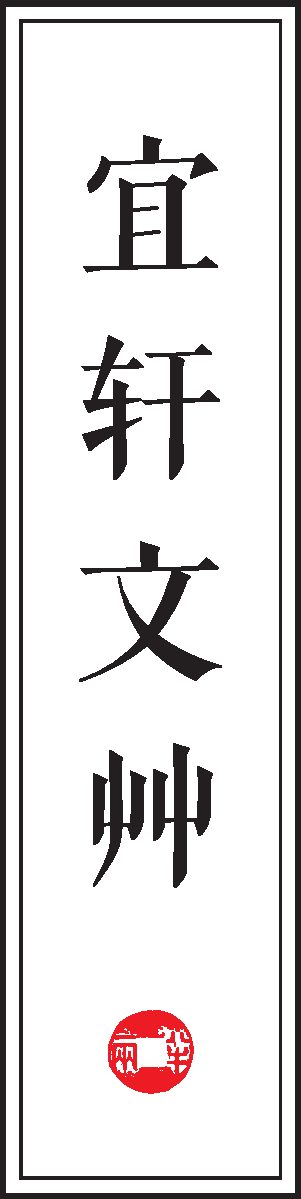
\includegraphics[height=125mm]{image/yxwcfront}
	\end{center}
\end{titlepage}
\clearpage
\pagestyle{empty}
\mbox{}
\clearpage
% 目录页	
\pagenumbering{Roman}\setcounter{page}{1}
\tableofcontents
\pagestyle{plain}

\chapter{闷~~骚}
\thispagestyle{empty}
\pagenumbering{arabic}\setcounter{page}{1}
\clearpage\mbox{}\thispagestyle{empty}

\section{踏雪访梅}

\blfootnote{高中时代旧文,青涩年华记忆。}赏梅的去处,要数着江南的几处胜迹了,金陵吴王坟,姑苏香雪海便是其佼者。也曾诣吴王坟,也曾游香雪海;梅英如海,人影如潮。心里总觉着不若许久以前踏雪访梅的意趣。

家乡的老辈人总以为从腊月二十三祭灶神开始算过年,除夕祭祖祝福,初一祭天地,初五奉财神,直到元宵才算过完年。元宵节却不是正月十五那么简单,正月十三就要扎青门,家家户户张灯结彩,十五闹元宵“一夜鱼龙舞”,十八晚上收灯,十九开市,年才真的叫过完了。前前后后有一个月,我是受不了这样的喜庆的。每年回家过年,也没有什么新意,只是父母年纪大了,回家看看,聊表孝之道罢。初一到初五走亲访友,落不得半日闲功夫。那一年天公作美,初一到初五都是晴天,走亲访友倒没有吃什么苦头。

初八阴了天,家乡人的说法是龙翻身。初十飘起了大雪,纷纷扬扬,真可称得上一个“紧”字了。自小在江南长大,第一次才知道什么叫做鹅毛大雪。这是一场江南少见的大雪,据老辈人讲百年也是难遇的。地上铺满了雪,柏树压折了树冠,垂头丧气地立着。不过对我来说,这的确是一场好雪,不必做那些年后的回拜,倒也清闲自在。捧着缭绕烟雾的清茶,诵诵诗书也不必红袖添香,自有案头凌波侧目顾盼。或者隔着窗户赏看雪景,古人有打油诗云:“江山一笼统,井上黑窿洞;黑狗身上白,白狗身上肿。”真不为过也。这样的清闲不知过了几日。

一夜,坐于案边诵“疏影横斜”之句。忽觉耳边几声啁啾的鸣叫,甚是诧异。推开窗户,清寒扑面而来,沁入心脾使人神清气朗。雪停了,天晴了,银轮悬在苍穹,乱琼散于原野,交相辉映,人间的灯火黯然失色,不忍多看。今夕何夕,天上人间。广寒宫中的嫦娥是否起舞。熄了屋里的灯,静静地享受这荡漾清辉的世界,清寒往肌肤深处行去,却不甚冷。“疏影横斜水清浅,暗香浮动月黄昏。”不觉诵出了声,惊醒了自己的梦。想起梅花一定开着。便着了木屐扎上草绳,出了门,向屋后不远处的小山走去。

路上的积雪蓬松而柔软。足有一尺多厚。使劲跺跺脚,发出了“嘭、嘭”的声音,惊了栖于枝头疑是白日的麻雀,扑喇喇地乱飞。心底遗忘许久的童年的顽皮露出了得意的笑容。只是双脚却深深陷在草地里。皎洁的月色下,树木的身影怪异地映在雪原上,有如妙手偶得的水墨。

这山其实称不得山,约摸十多层楼房的样子,只能算是个大土堆。山脚有一条婉延曲折的小溪,夏日里农家的孩子常在那儿捕捉小鱼小虾。溪头的垂柳遮出一片浓荫,远处不时传来牧童的笛声,那是个读书的好去处。此刻溪头一样积了厚厚的雪,只有溪水仍然默默地流动,显示出一种墨玉的颜色,看起来有些静秘。小山有个鲜为人知的名字“鬯岭”。那是一次夏季暴雨冲出一块怪石,上面刻着这两个字,字迹早已漫漶了,依稀能辨认出来,遒劲而雄浑,颇有史晨之遗风。边款荡然无存,不可考当年的情致了。也许当初本无边款,倒是我这个后来人凭空多了几分遗憾而已。翻了《康熙字典》才知道“鬯”是祭祀用的一种谷物酿成的酒,念畅的音。只是不知道这个小山起名“鬯岭”当初是缘何而来。是否恰恰是指着山下的农田而言的谶语,或许初建之时就已了然免不了的结局了。溪上有座汉白玉的小石桥,已经残破不堪了,而此时那平日里掩饰不住的往昔精致和周围田野中偶尔能看到的柱础,全部的怀旧都覆盖在积雪之下,兴与衰的感叹了无痕迹。

小心翼翼地走上山去,不能闲庭信步了。得看着脚下,辨清道路,跌了眼镜,是无处可寻的,颇有些狼狈。其实,路在平日里就是没有的。大雪覆盖之时,更是难寻。鬯岭之上另是一番情趣。几株梅树错落地立于乱石之中,然而此时的乱石失去了棱角,涌动出奇怪的模样。盘曲的枝干积了雪,添了几分婉转与圆润,蓦然横空,映在银色的雪原之上有如矫龙游于云海之中。淡淡的清香随着清寒的空气飘了开去。花是不容易辨认的,洁白而柔软的花朵与冰雪凝成一片,真不知道是梅花香还是那冰雪更芬芳。有如此的冰雪,有如此的清馨,真当起舞了。

邀明月,邀寒梅,与我同舞。林逋,你若有灵,来这荒郊雪原与我同访这孤傲的梅花吧!寒梅,你若有知,当为我开放!今夜,有月如水;今夜,有雪如琼;今夜,有梅如影。他年还有这样的佳景否?

此后多年,也曾到过许多地方,喧闹的梅海,喧闹的人潮,于我总觉得不关什么事体,有谁同我去顾盼那鬯岭上的孤梅。每年回家乡总要访那几株梅树,只是何处能得瑞雪,何处能得满月。
\section{中秋}

\blfootnote{一九九六年。}虽然,白天还是夏日般的闷热,夜晚寒意侵入衣底的时候,便觉着秋日已经到 
来。书上常说的“金秋”,在合肥其实是看不到,夏日的浓绿不经意就变成了褐色, 
无论如何也不能让人有一种愉悦的感觉。只有晴朗的天空中显现出的明净的蓝色, 
倒还爽心悦目。行人的夏装,依旧潇洒;女孩的裙裾,依旧翩翩。只是商店门口巨 
幅的月饼广告,大肆地宣告着秋天的到来,不肯让人多一些夏日的梦。 

翻一翻日历,才知道中秋节没有几天了。一个人在异乡,节不节的无所谓,月 
饼也是可有可无的。团圆只是在梦里的快乐。 

月饼的来源,据说是元末农民起义时传递消息的一种有馅的圆饼。起义者们提 
着竹篮,竹篮里放着刚刚烤出来夹着起义消息的圆饼,装着过节走亲戚的模样,向 
关卒躬身哈腰地走过一个又一个关卡,心里却恨恨地说:“待得老子事成,杀你个 
直娘贼。”至于以后如何有了团圆美满的象征意义,我是不大清楚的。想来大约是 
由月圆到饼圆的罢,果然这样的话,始作俑者,怕的要是东坡了。如今,月饼好象 
已不仅仅只是中秋节必备的美味点心了,正所谓是“吃的不买,买的不吃。”商店 
里陈列在橱窗里的月饼包装得花花绿绿的,正如青楼的红尘女子待价而沽,一个要 
卖上百;早知现在,月饼这玩意还是扔进水沟的好。几百块钱的月饼吃在嘴里,真 
不知道是什么滋味。虽然,有月饼我还是要吃的,不是上百的也不是几十,两 
三块钱已是不错的了。
 
在记忆中,最好吃的月饼是母亲做的芝麻糖馅糯米面饼。小的时候,家里不是 
很宽裕,食品店里的月饼只能买上一两个孝敬奶奶。母亲想尽一切办法让我和妹妹 
高兴。在农村的舅舅过年带来的一点芝麻,放在锅里炒得满屋飘香,再放在铁臼中 
舂碎,拌上白糖,就是芝麻糖馅。我和妹妹早已馋得咽口水了。糯米面也是买一点 
廉价的糯米,淘洗干净,泡上一天,也放在铁臼中舂细。比不得现如今商店中,塑 
料包装袋中的水磨元宵粉。对于那时的一般家庭来说,已是一样奢侈品了。刚刚烤 
好的芝麻糖馅的糯米饼我可以一下子吃三个。直到今天我也不能忘记,融化的糖汁 
裹着芝麻粉流出来烫着我和妹妹的嘴,母亲脸上的苦涩的笑容。如今母亲再也不会 
为月饼发愁。只是这月饼吃在口中,早已没有什么感觉了。

江南这个时候所习见的美味,都是水中生长的肥嫩的菱角、薏仁之类的。用长 
长的树枝在塘中随意挑起,剥去外面的皮,含在嘴里凉凉的、甜甜的,慢慢地化作 
满口的清香,没有一些些渣滓。琥珀色的封缸老酒更是“味轻花上露,色似洞中春。 
”天上的圆月在淡淡的浮云中徜徉,印在水中,印在杯中;清凉的微风拂过水榭, 
银色的光漾漾地散在水面。应该是最好的享受了。 

在今天的日子里,又会有谁“举杯邀明月”。远离故乡的日子,中秋如同一个 
又一个普通日子,平静而又平静。也许明年我该回家过一个中秋。 
\section{化蝶}
	
\blfootnote{大学毕业之后,大约一九九五年前后。}庄子曾经做了一个梦,梦见了自己变成了蝴蝶。
	
蝴蝶曾经做了一个梦,梦见了自己变成了庄子。
	
上面的两句话,第一句好懂,第二句着实有些让人莫不着头脑。当初,庄子或者蝴蝶或者庄子和蝴蝶也不知道第一句是真还是第二句是真。
	
江南吴越地方的传说却是有化蝶的,不是如此地不明白,而是明明白白地化蝶。这便是著名的民间传说:梁山伯与祝英台。不过,我很奇怪的是两位主人公会有这样奇怪的名字。年纪轻轻何以敢称“伯”,若说是排行也应该在中间。“英台”二字,知识隐约觉着从南朝某处诗歌中得来,手头没有资料,想考证也只好作罢。传说中祝英台之父是否是饱学大儒,也没有明言,不过说得明明白白的其父是个员外。“英台”二字好象也就没有来由了。也许以讹化讹,便这样说开了;话说回来,吴越的方言也着实难懂,就同音替代也未可知。我想也不必象非要找出“杞良妻”就是“孟姜女”的来源那样。大家都这样说,便这样说罢。
	
梁山伯与祝英台的传说,在吴越地方不只是大家所熟知的,还有许许多多的故事,要是都说出来大约可以写成大部的砖头书。只是其中之一我颇感兴趣。说是祝英台有一个哥哥,有哥哥就少不了有嫂子。大多数的民间传说中,姑嫂照例是合不来的,这里也没有例外。既然祝英台是个“美丽动人的好姑娘”,嫂子当然是个“恶毒凶狠的坏女人”。这里我要声明:这是照着老例讲的;至于,祝英台是否真是个“美丽动人的好姑娘”,嫂子是否真是个“恶毒凶狠的坏女人”,这里暂且这么说罢。
	
祝英台要去杭州读书。她父亲是反对的,嫂子也是反对的。不过,既然其父爱其女如掌上明珠,也是扭不过的。嫂子反对的理由是:一个未出阁的女子,如此便是不守妇道要如何如何了。为了不象方鸿渐那样如何了女学生的耳朵,这里就不明说了,恐怕有人比我还要明白得多得多。祝英台便指着后园的一丛牡丹说:花败便如何等等。嫂子自然是不服气的,祝英台一走,嫂子就用开水烫牡丹,不但没有烫坏,反而越发地茂盛了。情急之下拔出根来用火烧,再插回地里去,地上的部分是不能动的,否则是要露馅的。没想到烧过之后不但没死,居然烧出个“焦骨牡丹”的新品种来。祝英台的嫂子做了一次牡丹品种改良的大功劳。要由此来说明祝英台的冰清而玉洁。不过,这里有个可疑之处,牡丹从不生于江南,祝英台的籍贯便不会是吴越地方了。
	
前面说了祝英台要去杭州读书。要读书非去杭州不可,俗话说得好:“上有天堂,下有苏杭。”杭州是繁华闹市,旅游胜地。当然现在的浙江大学是很好的学校,但当时呢?不得而知。不过,大儒先哲结庐于偏僻之处,可以推而及之,杭州准确地说当时的杭州是否真是个读书的好去处。那么祝英台要去杭州读书的目的,大家自己去想象罢。
	
回过头来看看梁山伯。至于梁山伯,我不知道,他是真傻还是假傻。若是真傻,便是迂腐,这样的人本不值得爱的;若是假傻,便是情场之高手了,按现代的说法叫做“吊”。十里相送,祝英台以九妹为掩暗许终生,梁山伯欣喜若狂;而祝英台所指的九妹便是自己,梁山伯若是以为祝英台为男子, 那么凭什么理由认为“九妹”就是个好姑娘,能够成为自己的好妻子。梁山伯若是假傻,其手段是高明的,一方面既符合了道德的规范,一方面又有了佳人为妻,两头两头逢源;这样的话,十里相送,缠绵悱恻,倒是非常有趣的。
	
祝英台的父亲,传说中是个员外,员外其实就是地主老财,决不会是个饱学大儒。爱其女如掌上明珠,好象也是没有理由的;若是真的爱其女就不会因为县令的压力,而应承这门婚事。看来,爱财才是真的,爱其女不过只是当其是一个玩偶罢了。祝英台作为一个女子违反礼教,这件事,是当时的道德规范所不允许的;因而,祝英台的嫂子的反对当然是有理由的,而且是正当的理由。其实,牡丹根本不用去烧,“嫁出门的姑娘,泼出门的水。”祝英台不会分其家产,反正妆奁是少不了的,清白也好不清白也好于她是乌有关系的。只是这传说要说祝英台的好,定要找个局外人来垫底罢。
	
令我奇怪的另一件是:既然有了楼台会,想必是可以私奔的。司马相如和卓文君的私奔是个佳话,那么,梁山伯和祝英台的私奔也应该是个佳话。结果呢?梁山伯郁郁而亡,祝英台投进了坟墓。不过,如果真的是马家迎亲,壮丁一定少不了,正要趁着机会巴结县太爷,如何连一个弱女子也拦不住,祝英台毕竟没有祥林嫂那样的健壮。于是,祝英台投进了坟墓,与梁山伯双双化为了蝴蝶,翩翩起舞了。
	
写到这儿,我想起了与此相类似的一个西方著名悲剧《罗密欧与朱丽叶》。结果一样都是一个“死”字,但导致“死”的原因却有天壤之别。朱丽叶的假死是要躲过出嫁,其目的是要活下去,和罗密欧偕老的。只是阴差阳错导致两人双双殉情。要注意的是:朱丽叶把“死”作为一种手段,以达到和罗密欧的结合;而梁山伯看来根本没有打算活下去,这是一个多么大的差距。生命是可贵的,如果没有了生命,还能够谈论什么?更不要说“爱情”了。当然牺牲是不可避免,也不应该避免,那是为了更多的生命。就个人而言,生命难道不是最可宝贵的吗?
	
然而,人的意志如何坚强,也是难以承受岁月的磨砺。因此,没有人能够在没有结果的爱情之后,说“永爱一人”。故事在此以“死”作为终结,是再好不过的了,坚贞不渝的爱情便越发显得高尚了。人的生命相较于此,也就无可宝贵的了。“死”便成为一种逃避,逃避美丽爱情故事后面难以掩饰的尴尬境地。
	
国人的自我安慰,的确是举世无双的。现实里不能够实现的,可以等到来世。生不能为夫妻,死后为蝴蝶,世人便管不着了。逃避现实,国人的经历太多了。
	
当然,梁祝的故事主题是一个几乎永恒的主题——爱情。宝黛的爱情,得出了一个“空”字,我真的不明白,象贾宝玉这样一个热爱生活的人,居然会跟随和尚道士离家出走。梁祝的爱情得到的是一个虚幻的团圆。人类的想象是任何势力所不能遏止的,于是,想象便是一个绝好的去处。现实是残酷的,想象可以按照人们的意志去安排。我不知道,玉皇大帝是否会干涉这对可爱可怜可敬可悲而又太脆弱的一对蝴蝶的爱情。
	
梁祝追求的是否真是人们所说的“自由恋爱”呢?至少在我看来不是这样的。祝英台并没有直接说出来,而是假托并不存在的九妹,归根到底是要符合礼教的,不恰当地套用一句话叫做“曲线救国”。如果成功了,便是佳话,“才貌双全,珠联璧合”;如果不成功,便是悲剧。然而,悲剧却长了一条不折不扣的老鼠尾巴——化蝶,所有的矛盾就这样解决了,倒也快刀斩乱麻;无论怎样,在人们悲愤之余,来一条手绢擦擦眼泪为化蝶而欣喜,总是件好事。于是,悲剧就这样地淡化了,传说也因此而美丽起来。当然杭州的美丽景色为这个美丽的传说又添了一层美丽的外衣,恰如一个愤怨的美人,越发地标致起来。人们便忘记了美人的愤怨,只是看着美人的容貌发呆。
	
倘若当初司马相如和卓文君的故事也是以悲剧而终结的话,按照国人的传统必然有个同样的类似化蝶的尾巴。
	
我们所需要的不是幻想而是现实和由现实推及的理想。现实需要承认,但现实更需要我们去改变。梁祝充其量不过是企图钻一个现实的空子,实际上企图没有实现。倘若,梁祝真正是为了自己的爱情,私奔应该是最好的解决办法。可是对于梁山伯与祝英台来说,这是一个灾难,祝英台能否象卓文君一样当垆卖酒,梁山伯能否去做店小二,我是不敢说的。建筑在空虚的基础上的爱情,是无法存在下去的。设想梁祝二人如果真的“有情的人都成了眷属”,浪漫的爱情只可能建立在衣食不愁的基础上,只可能是有钱而有闲的。
	
马文才这个角色,不应该不提的。传说中的马文才,相貌猥琐,胸无点墨,是个仗势欺人的额势力的代表。马文才的出现不过是要悲剧的悲伤更浓一点,让人们的泪掉得更多一点,从而使那条老鼠尾巴看起来更漂亮的一点而已;即使没有马文才这个角色,梁祝的故事就能够圆满吗?
	
其实,梁祝的故事并不一定有过,只是国人逃避现实的又一个顶峰。可以安慰许多并不幸福的人把幸福寄托在天国,寄托在来世;可以省却许多反抗和反抗带来的混乱。不能不说,为了太平而叫人们把追求放在谁也不能证明的幻想之中,的确是个好方法。直到现在还是有人这样去做。
	
社会进步了,思想解放了,天国的幻想也就没落了,被人们抛弃了;然而人们把理想也一同抛进了垃圾堆,只在注意“利”字。有钱的浪漫成了时髦,有钱的潇洒成了时尚;钱便决定了一切,决定了生命。人们打破了礼教的枷锁,又给自己套上了一个铜臭的枷锁。而国人的眼光却没有多少变化,能够打动人心的仍然是那些“不食人间烟火”的“金童玉女”之间的“爱情”,是美丽的,是缠绵的;传说中的美人更加妩媚了,更加挑逗人们心中的那一块小秘密了,挑逗得人们越发地舒心顺气。悲剧的 影子也不存在了,矛盾也不存在了,翻过来倒过去, 只剩下了“情挑”二字。
	
于是,少男少女纷纷追着时尚去了。悲剧就这样从我们的生活当中悄然而去。梁祝的故事只是故事而已,留不下什么东西了,人们谈论起来只是一个美丽的民间故事,一个愤怨的美人而已。其唯可利用的不外乎两种:换汤不换药和换药不换汤。梁山伯成了武林高手,英雄救美的故事,依照传统又演绎下去了,给“天下熙熙,皆为利去;天下攘攘,皆为利往”的人们增添一些笑料,让人们在笑的时候,忘记一只在自己口袋里掏钱的手,这便是成功了。于是,想象力便是捞钱的 本领。苦苦追求理想的人便成了“呆头鹅”。
	
梁祝的故事到化蝶便完了。我们来设想一下,这后面会发生一些什么事情。蝴蝶是否就自由了,不必说天上的玉皇大帝,来了一只黄雀,吃了一只蝴蝶,这样故事该如何演下去?是不是,另一只蝴蝶也要自投雀口?然后再化作什么呢?只能化作鸟粪了。我想不会有人允许我这样设想下去的,我自己也是不能够的。看来人们的想象还没有达到一个一劳永逸的地步,化作神仙不是更好。我不知道这样是否还能够象化蝶一样动人。
	
面对这样的一个故事,我们得到了什么呢?我是不知道的。悲剧没有了,只剩下了美人。逃避仍然存在,只是不能逃往化蝶的幻想之中去了。“发财”的幻想越来越深入人心了,于是人们更加“岌岌可危”地护住自己的口袋,而伸手到别人的口袋里掏钱的想象力越发地膨胀起来,落到个人身上的责任就越来越少了。
	
梁祝的悲哀已没有多少人理会,化蝶的传说,就成了博物馆里的精品了。在欣赏之余,可以作为“高雅”的象征。梁祝的传说,当初何曾高雅过,民间传说,村鄙俗语罢。
	
也许,果真是两只翩翩起舞的蝴蝶做了这场梦。庄子若是有灵,该有何想?我只好说不得而知了。
\section{呓语}
	
\blfootnote{二〇〇三年,短暂无聊赖的日子。}\textbf{之一}

\pskip	
每天都告诉自己一定按时吃饭,每天都胡乱找点什么。
	
每天都告诉自己一定打扫卫生,每天都面对满屋子地垃圾。
	
每天都告诉自己一定要戒烟,每天都微笑地对着楼下杂货店老板说来两包。
	
每天都告诉自己一定12点睡觉,每天都要听到窗外马路对面卖早点的小摊子生火的声音才知道天就快亮了,该睡觉了。

\pskip	
已经忘记早晨太阳如何升起。

已经忘记满天的繁星时什么样子。

已经忘记哪一张CD曾经是我的最爱。

已经忘记我来这里干什么又要去往何方。

\pskip
记忆中,只有黯淡的黄色和黑色。

昏黄的灯光,有气无力地照亮黑夜中破旧门楼的前一小片地方。门楼前的物件,还是当初的模样。

已经不是当初的模样,只有破旧摆在眼前。路边的窗户,亮着灯光,传来POP的节奏,徘徊在破旧门楼前面的旧巷。这不是雨巷,不会碰见撑着油纸伞丁香一样的姑娘。

旧的港口,还能停泊旧日的船只;旧的街巷,还有什么会路过此地。

\pskip	
\textbf{之二}

\pskip
总是喜欢一个人看着微风中瑟瑟的无名的白色的小花;

总是喜欢一个人在微雨中徘徊在水边任柳枝摇摆在我的面庞;

总是喜欢一个人远远聆听古寺里传来的袅袅梵唱;

\pskip
不知道什么时候开始,我很享受寂寞。一个人的夜晚,翻检着落满灰尘的CD,翻检着泛黄的书页,桌上的清茶,冒着热气,外面的世界已经不再存在。

佛陀在灵鹫山上捻花微笑的时候,已经在梦中种下了毒药。去赞叹佛陀的智慧,还是去诅咒佛陀的恶毒?

曾经一个人,拖着行囊,走过虎跳峡峻峭山崖上的小路,峡谷中飘荡的风,吹着我的头发,蓝得不能再蓝得天空,总是有一种纵身而下的冲动,我也不知道我在寻找什么。

\pskip
窗外夜色已经浓重,我闻见马路对面卖早点的小摊子生火的木材燃烧的味道了,该去睡觉了。
又是一个享受寂寞的夜晚。

\pskip
\textbf{之三}

\pskip
醒来的时候,已经是下午时分。才是周五,周围很安静,只有公共汽车电脑报站器的声音:乘客您好,欢迎乘坐6路公共汽车,本车开往大兴镇。很清晰地钻进我的耳朵里。平时没有注意过的东西,此刻居然这样清晰实在,彷佛能触摸到它的影子。

\vspace{0.75em}
起来之后的第一件事情,摸索着烟盒,空了。于是靸了拖鞋,下楼,微笑着对着杂货店的老板,一如既往:来两包。点燃香烟,泡上一杯瓜片,慢慢咂着,我才算清醒。

\pskip
也许是清醒吧,也许还是在梦中。庄子不知道是庄子梦到蝴蝶,还是蝴蝶梦到庄子。我不是庄子,我也不知道庄子是否知道是庄子梦到蝴蝶,还是蝴蝶梦到庄子。我也不知道是否是什么怪样子的东西梦到的我。
	
\pskip
\textbf{之四}

\pskip
十二点已经过了半个小时,拿起手机又放下,放下手机又拿起。不知道是想拨一个电话,还是希望接到一个电话。记忆已经模糊不堪,梦里的旧巷淡如泛黄的照片。那扇窗户是否还亮着灯光。

\pskip
干白,在杯中就和我的记忆一样的泛黄。CD,在屋里就和我记忆一样的模糊。曾经水边的徘徊不再,只有酒和机器陪伴我的夜晚,今夜是否会有梦?不知道,是希望有梦,还是不希望有梦。没有梦的日子,远离爱恨,却是难耐的寂寞。有梦的日子,远离寂寞,却是理不清的爱恨。
	
\pskip
还是翻检翻检书吧,幽幽地吟了诗词,或许能不再思考这样到处都是正确答案的难题。或许是注定的寂寞,“梦里不知身是客,一晌贪欢”,一出口,就已然后悔。

\pskip
夏日无风的日子

该用某种东西来结束

这摇弋的渴望

\pskip	
守望在杨柳岸边

于孤寂的夜晚

一任冷雨扑打窗棂

\pskip
月的朦胧

依然弥漫在这多情的季节

我却在寻找柳絮飘飞的家园

\pskip
\textbf{之五}

\pskip
天气又开始阴霾起来。我不晓得到底是否喜欢下雨。

\pskip
记忆里,总是回绕初春细雨中的柳色和渔歌。最爱江南细雨微蒙,独自漫步在河边的柳树下,任柳枝摇曳发端,任渔歌回荡耳畔,任雨丝吻在面庞。初春时刻虽是清冷,却也有无限的温柔。

\pskip
记忆里,总是回绕夏日暴雨中的呼喊和痛苦。暴雨中的呼喊只有两个人听见,暴雨中的痛苦只有两个人知晓。天地不应,人事尤远,世事无奈,“这次第,怎一个愁字了得”。

\pskip
而今,已然不再细雨漫步的闲趣,也不再有暴雨狂呼的痛苦,不再有年少的狂放。有的只是千篇一律的说辞,有的只是习惯而自然的职业般的微笑,有的只是所谓成熟的稳重。

\pskip
窗外传来孩子们奔跑的欢闹,生疏了,生疏了。
\section{荠菜}
\blfootnote{二〇〇四年。}转眼油菜花开,想着美味的青菜是没得吃了。在菜场里转了几圈,居然没有什么可以下口的东西,从菜场出来,篮子里不过一块豆腐,几个蘑菇,也是美味一格。

“老板,荠菜可要?”菜场门口一位五十来岁的妇女,面前一块塑料布,堆着一堆深绿色的植物。

荠菜?好东西来的。蹲下身,抓起一些在鼻子底下嗅嗅,清香非常。“可是野生的?”其实看看这深深浅浅、大大小小的荠菜,早就知道不会是地里种的。

“我一大早从河沿上挖来的。你闻闻,你看看。”

一会儿,篮子里多了一大捧荠菜。一路思索如何打发了这清香的荠菜。

\pskip
小时候,老师提起荠菜,就是旧社会如何贫穷,如何靠野菜充饥;父母提到荠菜,就是三年自然灾害,荠菜都吃没了。结果,自小就对荠菜没有好感。记得第一次吃荠菜,是妈妈包的荠菜饺子,原以为不会好吃,吃了之后才知道味道鲜美,他物难及。

对荠菜的认识还是在中学,我与同伴相约去郊外看早春的梅花。行进途中,看到几位老人在河边挖掘一种绿色的植物,大家好奇簇拥上去,七嘴八舌问了开来。“这个是荠菜。你们这满地都是荠菜。”仔细瞧来,一种嫩绿花白色的植物依地而生,它叶子形同锯齿,又像羽状一样分裂,清香扑鼻。于是大家不约而同地采摘起来,没有工具,就用手掐。不一会儿,手疼腿麻。四五个年轻人却没有那位老者来的利索。

\pskip
采食荠菜,古有先行。陆游有赞:“日日思归抢蕨薇,春来荠美忽忘归。”《本草纲目》中称荠菜为“护生草。”顾禄的《清嘉录》亦有:“荠菜花俗呼野菜花,因谚有三月三蚂蚁上灶山之语,三日人家皆以野菜花置灶陉上,以厌虫蚁。侵晨村童叫卖不绝。或妇女簪髻上以祈清目,俗号眼亮花。”可见,荠菜不仅有食用价值,还有药用价值,明目、利尿、解热、止血,据说常食荠菜还有美容之功效。农历二月初,村旁、地头、溪边或草地、麦田中,荠菜便露出了嫩嫩的尖,只那么一点点绿,就让寒气未消的大地充满春意和生机。荠菜长得快,仿佛昨天才露尖尖角,今天就已亭亭玉立,明天就会挺起长长的茎,顶着洁白的花。

\pskip
荠菜的吃法很多:将荠菜剁碎,用纱布滤去水分,与肉馅、适量盐、味精和在一起,可以蒸包子、包水饺、包小馄饨,清香扑鼻,口感极佳;还可以在滚水中烫一下捞起来,用香油凉拌,吃得满嘴的鲜香;与豆腐一起烧清汤,色泽一青二白清爽怡人,口感清淡舒适;与肉一起炒、煮荠菜粥等都可以,味道浓烈奔放。

而我却是喜欢荠菜豆腐圆子。荠菜开水焯过,细细切了,盛在白净瓷碗,很是好看。蘑菇加一点盐水煮开,已然柔软,细细切了,却是暗暗的灰色,煮蘑菇的水不要倒掉。豆腐加盐小火略煮,细细切了。细细切了?我没有这么好的功夫,不用切,用手捏碎就好。好了备料已经齐整,炮制开始。取大碗一只,放入豆腐,用手细细捏碎,加切碎的荠菜和蘑菇,加入芡粉、盐、糖、蛋青,顺着一个方向仔细拌匀。锅上坐油,火不要大,将豆腐泥捏成团状,下锅略炸成型。炸过的豆腐圆子下锅,加入煮蘑菇的水,加点盐、糖、料酒,小火煮透。火大了就散掉了。盛盘,汤在锅中略勾芡,浇在豆腐圆子上。于是,这荠菜豆腐圆子入了我口中,也不负放翁之美誉了。


\section{暮鼓晨钟九华山}

\blfootnote{二〇〇七年秋。}匆匆来到九华山,匆匆离开九华山,莲花佛国清静,也只不过是人世间的偶然而已。

到达九华山脚下已经是下午五点半了,天渐渐暗了,抬头看见一轮明月从九华山后升起,暮色中九华山青黛一般,没有雄浑,多的是柔美。如果不是周围其他人声音此起彼伏,真有点人间仙境的味道。

从山脚开往九华街的大巴蜿蜒行驶在曲折的山路上,司机很娴熟的转动方向盘,车内人随着车子左摇右晃,赞叹司机的声音不觉于耳,而司机无动于衷,想来这样的赞叹对他来说一天都有十多回,习惯了。

到达九华街的时候,已经六点钟,天色完全暗了下来。九华街上灯火闪亮,街上的游人不多,想来吃饭的吃饭,住店的住店。不见僧侣的影子,应该是做晚课的时间了。街边商店香烛、法器、山货等等琳琅满目。如果不是佛门法器成列,还真以为只是一个热闹的乡间小镇。即使莲花佛国也离不了物利二字。

本以为当晚就住在九华街,第二天一早上山。随行的朋友要做法事,与拜经台的主持联系说,法事早上五点开始。那时候索道还没有运行,问了路边的店家说,步行上山需要三四个小时,这样一来最迟凌晨一点就要出发。于是决定现在步行上山。店家听说我们要步行上山,一脸惊讶。

买一张导游图,打着手电筒,顺着石阶,开始了夜上九华山的旅程。离开了还在喧闹的九华街,夜晚的九华山其实很安静。月亮还没有完全升到天顶,手电筒的光线范围很有限,除了照亮的一点山路,周边的漆黑一篇。开始的路程不算艰难,山路逐渐陡峭起来,还真有点吃力。心想,该好好锻炼锻炼了。

山路越来越陡峭,抬眼是看不到头的石阶,只有埋头一级一级地上。一路上,隐约听见寺院的钟声与梵唱。大约半个小时,来到一个山顶,查看地图,乃是回香阁。殿堂的灯火已经熄灭,只有偏房传来笑语,走近才发现是僧侣们聚集在一起看电视。僧人也不是不食人间烟火的。过了回香阁,山路一直往下,走了不久也就比较平坦了。月亮已经升高,透过树林洒下斑驳的银色。九华山标志之一的凤凰松,在月色下是另一种意境。过了凤凰松,真正开始了攀登九华山主峰天台的路程。石阶路在山间回转,一路上遇到不少大小寺院,大多数已经是人定。偶尔能听见用功僧侣的诵经和木鱼的敲击声。我已无暇顾及这些,只是希望早点到达山顶。月色中,一路景色只是朦胧。

到达拜经台的时候,已经是九点钟。如果不是中途在一个叫做竹海饭店的地方吃了一段素斋,估计八点也就能到了。庙门已经关闭,敲门,开门的是一个二十岁左右的年轻僧侣,把我们引到会客室。一位中年僧侣接待了我的朋友,约定了第二天早晨法事的内容。

早晨四点半钟,手机的闹钟响了。朋友和我赶紧起床,他是要去参加法事的,而我是不拜神佛的。来到大雄宝殿之外,殿中已经有僧人在撞晨钟,口中念着经文,殿前香炉亦已焚香在内。天上繁星点点,炉内香烟袅袅,殿中钟声悠扬,远处夜色朦胧,多少有些远离人间的味道。五点整,殿中僧人排列整齐,法鼓咚咚,木鱼铜罄,僧人诵念经文,算不得悦耳。虽然,听不懂念的是什么,平缓稳定的节奏也能使人心气平和。站在殿外看着朋友在僧人的指导下,跪拜、焚香。愿你的祈盼都能实现。法事历经一个小时方才结束。天色逐渐明亮起来。

朋友从殿中出来之后,决定登上天台,又是一段陡峭的石阶,上到天台的时候,太阳刚刚升起,映照着云霞,瑰丽无比。自然,朋友又要去焚香膜拜,而我看看四下风景。山上已经有很多人了,巨大的香炉里已经满是燃着和燃尽的佛香。站在天台四处看去,倒也有一览众山小的气势。

七点钟,我们回到拜经台,朋友去见了主持和尚。离开拜经台,我们决定前往十王峰,围绕九华山的几个主峰转一圈。从拜经台到十王峰的山路,明显与其他山路不同。路上堆积着落叶,看来很少有人经过了。路边散落着五颜六色的纸片,仔细一看,原来是藏传佛教中的风马,看来有藏人来此转山,达到十王峰顶的时候,更证实了我的猜测,峰顶的松树间缠绕着许多风马旗。

虔诚的转山人祈盼这些风马旗上的颂愿能随着高山的风飘至佛前,真是叹服。象我这样空手上九华山都已经觉得不堪,而虔诚转山人背负这些沉重的祈盼来到山上。转过十王峰却发现又来到了天台,已经累得不行了,转山头的计划只好取消,于是乘坐索道下山。索道只需要十多分钟就达到凤凰松所在的附近。而昨天晚上却花了将近两个小时才走完。

下了缆车,我们顺着石阶路返回九华街。山间错落着一些房屋,如果不是屋前的香炉表明这是寺院的话,和民居没有两样。

一路走过,忽然遇着一座庵堂,上写“心愿庵”,朋友步入庵内,跪拜不已。一位老师太从偏房走到堂前,诵念吉祥语句,执椎敲了三下铜罄。我那位朋友紧闭双目一言不发,我知道他在佛前说了他的心愿,愿佛祖保佑……

匆匆来到九华山,匆匆离开九华山,莲花佛国清静,也只不过是人世间的偶然而已。
\section{愿你的美丽光芒四射}

\noindent 亲爱的奕忻:

我的女儿,今天是你十周岁的生日。晚上的生日宴会,你和你的同学们、伙伴们一起表演节目、做游戏。看到你这么开心,爸爸真的很高兴。宴会结束回家之后,你还不能平息你自己的兴奋,不肯睡觉,要爸爸陪着你说话,说到你将来要上中学、上大学,说到要爸爸陪你去看国王十字车站,去看霍格沃斯城堡,去看金字塔……我们说了很多很多。爸爸知道,在你小小的心灵里已经有了大大的世界。夜深了,你终于入睡了,四仰八叉,睡相难看,哪有白天那个可爱小女孩的模样,但在爸爸的眼里你永远是最漂亮的孩子。

当你还在妈妈肚子里的时候,爸爸就有预感,你是女孩。在和你妈妈开玩笑的时候,总是说“小丫头”长,“小丫头”短,“小丫头”如何如何。你出生的那天正好是北京奥运会的第三天,医生说“恭喜,恭喜,是个千金。”爸爸的预感变成了现实。皱皱的小脸蛋,一双大眼睛忽闪忽闪地望着爸爸,小手还不老实地伸出襁褓,不停地挥动。爷爷奶奶都说你像我。女儿像爸爸,天经地义。爸爸知道,抱在怀里的你是爸爸一生中最可贵的宝贝,是爸爸一生的骄傲。从蹒跚学步、牙牙学语,到学会了自己吃饭、穿衣、洗脸、刷牙,到上学读书、学舞蹈、学古筝,你一天一天健康成长。到今天整整十年,你从肥嘟嘟的婴儿长成活泼可爱的小女孩。

你已经在甜美的梦乡畅游了,而爸爸却难以入睡,有很多话想对你说,想来趁着今天这个值得记忆的日子把爸爸想说的话都写下来。给你写一封信,也许是个好主意。不过在电子信息如此发达的时代,爸爸自己也觉得写一封信颇有些怪异。等你再长大一些,说不定会觉得写信真的很老土。

爸爸也曾想过,把你培养成什么样的人?我亲爱的女儿长大以后会是怎么样的女孩呢?科学家?医生?艺术家?还是文学家?记得在和你差不多年纪的时候,爸爸跟你的爷爷说长大要做科学家。爷爷告诉爸爸,他不会给爸爸定一个目标,一定要成为科学家还是其他怎么样的人。爷爷要爸爸自己确定自己理想和目标,他说,只要是尽了自己最大的努力,即使将来理想和目标没有实现,也“不会因虚度年华而悔恨 ,也不会因碌碌无为而羞耻。”这么多年来,爸爸虽然没有实现当科学家的理想,但是爸爸一直在努力,直到现在还在努力学习,为家人、为社会努力工作。

亲爱的奕忻,我的女儿,今天爸爸也像爷爷一样,不会给你划一道线、定一个目标,让你沿着这条线朝着这个目标长大。和爷爷一样,爸爸也希望你自己确定你自己成长的理想和目标,将来做什么工作、成为什么家并不重要,重要的是朝着你自己的理想和目标尽自己最大的努力,永不言放弃。

知道你名字“奕忻”的意思吗?“奕”取自神采奕奕,是美丽、光明闪亮的意思;“忻”是开心快乐、生机盎然的意思。爸爸虽然不会给你指定成长的目标,爸爸妈妈、爷爷奶奶都希望名字叫做“奕忻”的女孩美丽、快乐、健康成长。这个名字就代表了这个期望,也代表了对你的祝福。爷爷本来是选“欣”这个字,而爸爸更希望你的美丽、你的快乐和你的成长都是来自你自己的内心,决定就用这个竖心旁的“忻”字。

我想你会问:爸爸,爸爸,美丽、快乐和成长怎么会是来自内心?美丽不就是漂亮吗?遇到开心的是事情才能快乐啊?个子一天天变高就是长大啊?心藏在身体里,谁也看不见啊。亲爱的奕忻,我的女儿,爸爸知道你长大了,会思考问题了。想一想,我们可以说“这是一个美丽的女孩”,我们能说“这是一只美丽的小猫” 吗?不能,我们只能说“这是一只漂亮的小猫”。爸爸带你去爬山你很快乐,但是要你回家之后写篇作文,你还会快乐吗?肯定不会。姑姑家的海鹏哥哥长得很高了,是不是就是个子长高了呢?当然不是仅仅他长得比你高,是因为他懂得比你多,带你玩的时候知道照顾你,是不是很有爱心呢?

因为我们是人,我们不是花花草草这样的植物,我们也不是小猫、小狗这样动物。我们会思考问题探索世界,我们会判断对与错,我们懂得爱,爱国家,爱家人,爱朋友,爱一切美好的事物;而花花草草、小猫小狗它们都不会。

拥有魔镜、有着漂亮外表的王后,她美丽吗?不,她不美丽,她内心狠毒,想用毒苹果毒死白雪公主。被富翁叭哈收养的大林,养尊处优,有200个仆人伺候,他快乐吗?不,他一点也不快乐,好吃懒做,最后饿死在金子堆里。哈利波特的表哥达力,比哈利波特个子高,比哈利波特长得壮,他真的长大了吗?不,他没有长大,他只知道乱发脾气,只会欺负人。美丽和丑陋、快乐和难过、成长和幼稚,不仅仅是我们外貌的变化,更是我们强大内心的外在体现。

“爸爸,爸爸,我怎样才能内心强大,成为美丽闪亮、快乐成长的女孩呢?”爸爸在想你一定会问这个问题,因为爸爸知道奕忻希望自己快快长大。类似的问题,爸爸也曾经象你一样问过你的爷爷。你的爷爷没有告诉爸爸答案,只是说这个问题的答案需要爸爸自己去寻找。爸爸相信爸爸找到了答案,这就是自信、友爱和正直,是让你美丽、快乐和成长的真正的源泉。

自信,相信自己能够做到,但不是盲目的相信。自信来自不断的学习,遇到问题的时候去找出解决问题的方法,而不是被问题所打败。你的成长才会由你自己做主,而不是被问题所左右。太爷爷去世的早,爷爷小学毕业就去上了技工学校,没有继续读高中、读大学,十六岁就参加了工作。但是爷爷并没有因此放弃,一边工作,一边学习。在四十多岁的时候,还参大学函授学习,获得高级技师的职称。退休后还学习计算机、学习AutoCAD等工程设计软件。这就是你爷爷的自信。你应该还记得,你还没有上学的时候在家里调皮打坏了东西,都会说“爷爷修,爷爷修。”在你的眼里爷爷是万能的,如果爷爷不学习怎么会是万能的?

友爱,爱家人,爱朋友,爱自然、爱社会、爱国家,善待他人,在力所能及的前提下爱护帮助别人,你就会获得伟大的友谊。你自己应该已经能够体会友爱的含义,你有你“死党”,他们就是今天在你生日宴会上和你一起表演节目,做游戏的小伙伴们。将来你上中学、上大学还会遇到许多这样的伙伴。你们会互相学习、互相帮助,在成长的道路上陪伴在一起,而不是一个人去面对困难和问题。你的成长将丰富多彩。爱会让你更加自信,爱会让你的美丽从内心涌现,漂亮的外表和美丽的心灵在一起才会让你真正的美丽,才会你周围的人都会感受到你的美丽。

正直,遵守社会良知,明辨是非,要知道什么是错的什么是对的。人总是会犯错的。不要说像你这样年纪的孩子,就是像爸爸一样的大人也会犯错。犯了错不要紧,重要的是勇敢地承认错误,知道自己错在哪里,这样才不会再次犯同样的错误。这样你才能找到自己正确的方向,最终成长为对家人、对社会、对国家有用的人。

爸爸觉得,当你做到这三点时,你就会拥有一颗强大的内心,在你未来成长的道路上的一切困难都是纸老虎,你的自信、友爱和正直就是你最有力的武器,打败这些纸老虎,你就会成为美丽闪亮、快乐成长的女孩。

爸爸今天给你写了很多话。这些话,也许你还不能完全明白,但爸爸知道随着你一天一天长大,你一定会明白。爸爸虽然猜不出你的未来会是什么样,但是爸爸知道,爸爸一定会为你感到骄傲和自豪。

夜已经深了,窗外的夜空繁星漫天,一闪一闪,就像顽皮的孩子眨着眼睛。亲爱的奕忻,我的女儿,你一定就是那颗最亮的星星,愿你的美丽光芒四射。

\mbox{}

\leftskip=60mm 爱你的爸爸

\leftskip=53mm 二〇一八年八月十日

\chapter{潜~~歌}
\thispagestyle{empty}
\clearpage\mbox{}\thispagestyle{empty}

\section{致玫瑰}
\leftskip=25mm
\blfootnote{大学时代}
\noindent \\
如果你是玫瑰 \\
我不会把你放在温房 \\
\\
如果你是玫瑰 \\
我将聆听你的低唱 \\
风中的歌声,许是比曼陀林轻吟 \\
更加地撩人心扉 \\
\\
灯光下 \\
墙,在清茗的烟雾中 \\
退去,你的微笑,融在 \\
我的耳畔 \\
\\
雨中的传说,在匆匆岁月中 \\
成为老去的故事 \\
新的传说,在雨中诞生出 \\
无人知晓的碎片 \\
\\
等待一万年的歌声 \\
迷茫在人海的嘲弄当中 \\
就把这心掏出,在风中 \\
撕裂,就让这血,在风中 \\
飘散,就让这血,做你的 \\
衣裳,就让这血,浸着流浪的 \\
脚步,就让这世界都变成一般的颜色,血的 \\
暗红 \\
\\
如果你是玫瑰 \\
我会守望在你身边 \\
等待沧海的变迁,等待桑田的淹没 \\
等待你的绽放,就让你的色彩冲出 \\
你的心房,就让这血色的 \\
世界,一般的无光 \\
\\
如果你是玫瑰 \\
我要听着你,在月色下的低唱 \\
入梦,在梦里 \\
与你相拥

\section{粉色的梦}
\leftskip=25mm
\noindent \\
请拿起你的 \\
剑,刺进我的\\
心房,我要死在这\\
梦中,就死在这\\
粉色的梦中\\
\\
当最后一滴\\
殷红的,殷红的,殷红的\\
血,慢慢滑在你的剑尖,滴落\\
我就裂为千万的雪花,飘落,飘落在\\
粉色的梦中\\
\\
请抬起你的\\
头,看天上的残月\\
月华,如水,如冰,那就是我的\\
魂魄,如烟,如雾,飘散,飘散在\\
粉色的梦中



\section{山鬼}
\leftskip=25mm
\noindent \\
弃了你的薜荔 \\
  纫一枝秋兰 \\
  佩了你的鬓发 \\
低唱 \\
  左边,右边 \\
  左边,右边,幽谷,萦绕 \\
御风啊 \\
  乘了斑斓文豹,幽谷,徘徊 \\
\\
寻梦人啊 \\
入于山中 \\
去寻 \\
  寻一枝秋兰 \\
  佩了我的瑶琴 \\
低唱 \\
  左边,右边 \\
  左边,右边,幽谷,萦绕 \\
匣中,沉吟 \\
惊了碧桐裁制的瑶琴 \\
天啊,不假我 \\
弦已断,难应声 \\
\\
低唱,幽谷,萦绕 \\
  左边,右边 \\
  左边,右边 \\
\\
要循你的低唱 \\
  寻你的青丝 \\
幽谷,徘徊,低唱 \\
  左边,右边 \\
  左边,右边 \\
\\
筇杖,探不断的莽丛 \\
回首,凝眸,相视,与你的眼 \\
\\
散了你的发 \\
  做漫天的飞英 \\
揽天边的落霞啊 \\
  做你的衣裳 \\
\\
弃了你的薜荔 \\
  纫一枝秋兰 \\
  佩了你的鬓发 \\
御风啊 \\
  乘了斑斓文豹,幽谷,徘徊,离去 \\
\\
低唱 \\
  左边,右边 \\
  左边,右边,幽谷,萦绕 \\
\\
徘徊 \\
  是我的筇杖 \\
匣中,沉寂,追寻,无影 \\
徘徊 \\
  是谷中雾霭 \\
回首,凝眸,相视,与你的眼 \\
\\
漂泊 \\
  三千年的积尘 \\
要濯缨于沧浪之水 \\
\\
左边,右边 \\
左边,右边,徘徊,低唱 \\
\\
低唱啊,又起 \\
  惊醒了三千年的梦 \\
回首,凝眸,相视,在你的眼 \\
\\
匣中,碧桐裁制的瑶琴 \\
沉吟 \\
弦已断,不再鸣

\section{摸鱼儿·感怀}
\leftskip=20mm
\blfootnote{二〇〇〇年,瀚海星云。}
\noindent \\
看世间,无限风物,豪杰纵横可数。\\
凭栏吊古天涯客,高歌清扬我舞。\\
行觞趣,叹何苦,黄沙满卷云霄路。\\
挑灯醉觑,惊宗周稷生,应嘲两汉,铮骨埋碧土。\\
\\
南柯梦,空把光阴妄度,落的形销骨蹙。\\
吴勾掖绅策马顾,盟荐年少豪语。\\
轻落泪,但往来,莫问他年风飙处。\\
天下安住,任英名矫然,高节不废,山河更媚妩。
\section{归去之歌}
\leftskip=25mm
\noindent \\
之一\\
\\
你,告诉我\\
你,要离开,离开\\
去流浪远方\\
或归彼故乡\\
\\
我,无言\\
你,沉默\\
只有一个声音,在遥远,回响\\
归去,不如归去,归去\\
\\
是谁\\
在梦中,隐隐哭泣\\
是谁\\
在天空,写下记忆\\
是谁\\
在树梢,望穿秋水\\
是谁\\
在夜里,不停啼血\\
\\
是,忧伤的子规\\
还是,我忧伤的心\\
\\
缠绕在耳边的\\
还是,那个声音,遥远的\\
归去,不如归去,归去\\
\\
\\
之二\\
\\
还有泪吗?多少\\
轮回\\
爱,是那样的深沉\\
还能载多少\\
轮回的泪\\
\\
上辈子,我是\\
在山中见到\\
你\\
你是披着薜荔的\\
神\\
眼中的情\\
都化作你的泪\\
你的泪都化作你的歌\\
在我的眼\\
\\
上上辈子,我是\\
在林中见到\\
你\\
你是披着蒐萝的神\\
心中的泪\\
都化作你的情\\
你的情都化作你的歌\\
在我的心\\
\\
这辈子,我是\\
梦中见到\\
你\\
你是逍遥天地的\\
神\\
眼中的情,心中的泪\\
都化作你的歌\\
在我的梦\\
\\
还能见到你吗?还有\\
多少泪\\
能承载爱的舟\\
还有多少爱\\
化作飞天的雨\\
\\
还有爱吗?多少\\
轮回\\
泪,是那样的晶莹\\
还能濯多少\\
轮回的情\\
\\
归去吗?\\
归去你的故乡,还是\\
我的故乡\\
\\
归去吗?\\
归去你的归去,还是\\
天的尽头\\
\\
飘摇的人\\
只是放浪形骸,只是\\
归去乌有之乡\\
\\
下辈子,我是\\
在我的身边见到\\
你\\
你的曼妙\\
一如我,我所见,我所梦\\
下辈子,我的曼妙\\
一如你,你所见,你所梦\\
\\
下下辈子,下下下辈子\\
我不要在山中,不要在林中\\
不要在梦中\\
我只要我着你手\\
吻在你的脸\\
\\
归去啊\\
归去你的归去\\
归去啊\\
归去乌有之乡\\
\\
你的归去\\
是我的泪的故乡

\section{带脚镣的舞者}
\leftskip=25mm
\blfootnote{二〇〇三年}
\noindent(鬼魅)\\
我们是黑暗的神\\
旷野孤坟就是我们的殿堂\\
天下的一切\\
最终归于我们黑暗的神\\
\\
我们是生命的终结\\
生命只是短暂的绝望\\
只有我们才是存在的永恒\\
\\
旷野孤坟\\
摆满世间鲜血\\
豪华的筵席有谁能比\\
盛了鲜血我们干杯\\
歌颂我们自己\\
\\
啊,我们是旷野孤坟的神\\
豪饮吧,干杯吧\\
我们是旷野孤坟的主人\\
\\
\\
(诗人)\\
天上的神啊\\
我曾问你\\
是谁把这天上地下变得如此黑暗\\
你告诉我把心房\\
最后一滴热血奉献给你\\
就会获得渴望的阳光\\
\\
遵照你意愿\\
我已经奉献\\
寻找了世间的每一个角落\\
你曾许我的阳光\\
我未曾看见\\
\\
天上的神啊\\
为什么\\
没有了你的声音\\
你曾许我的阳光\\
我未曾看见\\
\\
心房里最后一滴热血奉献给你\\
我自己只是枯槁的灵魂\\
等待阳光的温暖\\
\\
天上的神啊\\
你听见了没有\\
你曾许我的阳光\\
我未曾看见\\
\\
\\
(鬼魅)\\
鲜血,鲜血,鲜血\\
枯槁的灵魂在说鲜血\\
他把心房里最后一滴热血奉献给天上的神\\
\\
哈哈,鲜血\\
哈哈,天上的神\\
哈哈,鲜血\\
哈哈,我们才是神\\
\\
天上\\
地下\\
只有我们\\
只有我们才是神\\
我们是享用鲜血的神\\
\\
我们是窒息生命的神\\
阳光已经死去\\
天上地下只有这旷野孤坟\\
\\
\\
(诗人)\\
为什么这样阴冷\\
我看见黑色的影子闪过\\
我只是枯槁的灵魂\\
在黑暗中飘荡\\
看不见阳光\\
\\
啊,你们,你们\\
是谁\\
\\
天上的神\\
我曾经奉献的神\\
为什么一言不发\\
你究竟是深沉还是无能\\
\\
你们为什么这样喧哗\\
黑暗的旷野\\
我看不见你们的模样\\
我的神\\
已经不在\\
我找不到曾许我的阳光\\
\\
\\
(鬼魅)\\
我们就是神\\
旷野孤坟就是我们的殿堂\\
我们就是天上地下的神\\
黑暗就是我们的阳光\\
\\
来吧,来吧\\
加入我们的行列\\
你会获得永恒的存在\\
来吧,来吧\\
享用鲜血\\
\\
\\
(诗人)\\
有一种温暖在干枯心房里跳动\\
啊,最后一滴热血\\
我离你竟然如此接近\\
啊,最后一滴热血\\
在金杯里激荡\\
\\
啊,我的神啊\\
你是否就在我的面前\\
为什么不再说话\\
\\
啊,你们是谁\\
心房里最后一滴热血\\
我奉献给天上的神\\
为什么在你们的金杯盛放\\
\\
\\
(鬼魅)\\
你崇拜的神就是我们\\
没有的世间的崇拜\\
我们怎会永存\\
\\
你奉献的心房里最后一滴热血就在\\
这金杯里盛放\\
许你的阳光只是谎言\\
\\
你,诗人\\
以前的诗人\\
你,诗人\\
枯槁的灵魂\\
\\
看吧\\
黑暗是我们的身体\\
我们就是天上地下的神\\
旷野孤坟的神\\
\\
你崇拜的神就是我们\\
天上的神已经死去\\
埋葬在这旷野的孤坟\\
\\
凡属阳光的\\
都要毁灭\\
黑暗的存在才是永恒\\
\\
来吧,来吧\\
加入我们的行列\\
就会获得永存\\
\\
\\
(诗人)\\
黑暗的阴冷让我发抖\\
你们骗了我\\
骗走我心房里最后一滴热血\\
我已经是枯槁的灵魂\\
\\
\\
(鬼魅)\\
你,昏聩的诗人\\
你,枯槁的灵魂\\
\\
只知道崇拜\\
从来不曾看过你自己的神\\
\\
昏聩的诗人\\
枯槁的灵魂\\
\\
加入我们\\
你就会获得永存\\
你自己也是神\\
黑暗的神\\
旷野孤坟的神\\
\\
\\
(诗人)\\
加入黑暗的行列\\
我就获得永存\\
\\
\\
(鬼魅)\\
枯槁的永存\\
黑暗的永存\\
\\
\\
(诗人)\\
没有阳光\\
就不会再有诗歌\\
没有诗歌的存在多么空洞\\
\\
黑暗的永存\\
黑暗的永存只是不变的枯槁\\
枯槁的永存只是黑暗的无穷\\
这旷野孤坟只有嘶哑的叫嚣\\
\\
\\
(鬼魅)\\
加入我们\\
分享我们的永存\\
最后一个枯槁的灵魂\\
你的阳光早已死亡\\
\\
黑暗的狂风\\
已经吹起\\
要最后一遍扫荡\\
世间所有属于阳光的\\
\\
黑暗的狂风就要到达\\
加入我们给你永恒\\
\\
你枯槁的灵魂\\
只会被黑暗的狂风破碎\\
归于黑暗之尘\\
\\
加入我们\\
分享我们的永存\\
\\
\\
(诗人)\\
我的阳光已经不在\\
\\
\\
(鬼魅)\\
你的阳光已经不在\\
离开我们\\
就是你最后的毁灭\\
\\
\\
(诗人)\\
我的阳光已经不在\\
离开黑暗就是最后的毁灭\\
\\
神啊\\
天上的神啊\\
你为什么死去\\
你是不朽永存的神\\
为什么死去\\
抛弃为你歌唱的诗人\\
抛弃诗歌对你的颂扬\\
\\
\\
(鬼魅)\\
你们,凡人\\
你们自己离弃了你们的神\\
在他的阳光下藏着\\
你们卑鄙的欲望\\
\\
成就了我们的力量\\
啊,黑暗的力量\\
\\
\\
(诗人)\\
神啊\\
死去的神啊\\
我已经没有诗歌为你哀悼\\
黑暗的世界里\\
我找不到我的阳光\\
\\
\\
(鬼魅)\\
加入我们的行列\\
不要犹豫\\
永存在黑暗的永恒\\
就满足你所有卑鄙的欲望\\
\\
\\
(诗人)\\
我已经找不到我的阳光\\
我是如此的彷徨\\
\\
\\
(鬼魅)\\
不要犹豫\\
黑暗的狂风已经吹起\\
枯槁的灵魂就要消散\\
\\
加入黑暗的行列\\
给你永恒\\
\\
\\
听,黑暗的狂风已经吹起\\
他的力量是多么的强大\\
\\
\\
(诗人)\\
听,黑暗的狂风已经吹起\\
他的力量是如此的强大\\
\\
\\
(鬼魅)\\
黑暗的力量\\
这就是黑暗的力量\\
\\
我们是黑暗的神\\
我们是旷野孤坟的神\\
\\
黑暗的狂风\\
横扫所有属于阳光的\\
成就黑暗的永存\\
\\
\\
(诗人)\\
听,黑暗中传来金属的碰撞\\
穿过黑暗狂风怒吼\\
\\
\\
(鬼魅)\\
听,黑暗中传来金属的碰撞\\
是怎样的碰撞\\
\\
\\
(诗人)\\
穿过黑暗狂风怒吼\\
这金属的碰撞\\
就像黎明的号角\\
多么嘹亮\\
\\
\\
(鬼魅)\\
是什么这样的响亮\\
旷野孤坟筵席上的金杯不会发出声响\\
\\
\\
(诗人)\\
黑暗使我渴望阳光\\
我看见你心中的明亮\\
对我黑暗中徘徊的枯槁的灵魂\\
就像我的阳光一样明亮\\
\\
\\
(鬼魅)\\
是谁\\
是谁还有明亮\\
世人的鲜血\\
都在旷野孤坟的殿堂\\
\\
\\
(诗人)\\
啊,舞\\
你在舞\\
啊,你是舞者\\
黑暗包围在你的周围\\
\\
你的心房\\
还有热血在奔腾\\
你在舞\\
\\
哗啦啦\\
金属的碰撞在你的脚上\\
你带着沉重的脚镣\\
\\
你在舞\\
带脚镣的舞者\\
\\
\\
(鬼魅)\\
带脚镣的舞者\\
带脚镣的舞者\\
他来自什么地方\\
他的热血还没有归于\\
旷野孤坟的殿堂\\
\\
快啊\\
黑暗的神\\
我们就是黑暗的神\\
夺了他的热血\\
成就黑暗的永存\\
\\
\\
(诗人)\\
看啊\\
带脚镣的舞者\\
\\
你的身边\\
是黑暗的叫嚣\\
你的身边\\
是黑暗的力量\\
\\
\\
\\
(带脚镣的舞者)\\
舞,是我唯一的语言\\
世间的一切我已经不能再说\\
我把自己流放\\
流放在世界的边缘\\
\\
世人都在崇拜天上的神\\
他们都已经忘记心房中热忱\\
心中热血逐步冷却\\
天上的神变得无力\\
\\
我把自己流放\\
流放在世界的边缘\\
\\
世人已经疯狂\\
分不清真还是假\\
天上阳光黯淡\\
宣告了神的死亡\\
\\
舞,是我唯一的语言\\
世间的一切我都不再述说\\
\\
世人都在崇拜天上的神\\
心中的爱\\
全部变得空虚无奈\\
人间的美好你们看不见\\
只知道对天上的神顶礼崇拜\\
\\
\\
(诗人)\\
你为什么一言不发\\
你没有什么要对我说\\
把自己流放了那么久\\
没有一点软弱\\
\\
你为什么一言不发\\
是否听见我发出的警报\\
是谁\\
让你带上沉重的脚镣\\
\\
我只是枯槁的灵魂\\
就要在黑暗狂风中消散\\
看见你头上的明亮\\
我知道还有希望\\
\\
\\
(带脚镣的舞者)\\
舞,是我唯一的语言\\
诗人,你\\
枯槁的灵魂\\
是否后悔\\
对天上的神的赞美\\
\\
舞,是我唯一的语言\\
脚上的镣铐\\
就是我的歌喉\\
哗啦啦\\
这就是我的歌唱\\
\\
舞,是我唯一的语言\\
诗人,你\\
枯槁的灵魂\\
是否听见\\
我的歌\\
\\
舞,是我唯一的语言\\
我带着脚镣\\
走过时光的隧道\\
从世界的边缘到另一个边缘\\
世界的中心\\
都是庸俗的迷乱\\
外表的高尚掩盖不了\\
虚假的邪恶\\
\\
舞,是我唯一的语言\\
我不会沉默\\
只是用我自己的方式\\
说着我自己的语言\\
听见的自然听见\\
听不见的也不需要听见\\
\\
舞,是我唯一的语言\\
这是我自己的流放\\
没有什么遗憾\\
没有什么哀怨\\
流放在世界的边缘\\
正好看\\
世界的堕落\\
天神的垂死\\
\\
\\
(诗人)\\
带脚镣的舞者\\
为什么你一言不发\\
\\
是的,我这个枯槁的灵魂\\
不值得你的顾及\\
我只是枯槁的灵魂\\
即将在黑暗的狂风中消散\\
\\
\\
(带脚镣的舞者)\\
舞,是我唯一的语言\\
诗人啊\\
感觉你干枯心房里曾经的跳动\\
你就会听见我的语言\\
\\
舞,是我的唯一的语言      \\
我不会再说世间虚伪的语言  \\
欺骗自己心灵的语言        \\
诗人啊                    \\
感觉你干枯心房里曾经的跳动\\
\\
\\
(诗人)\\
舞,你一直在舞\\
带脚镣的舞者\\
为什么你一言不发\\
\\
哦,心房,我的心房\\
干枯已久的心房\\
一种感觉\\
这样的熟悉,又是这样的陌生\\
我怎么也记不起\\
\\
我只是枯槁的灵魂\\
离弃生命已经很久很久\\
这种感觉\\
曾充满我年轻的胸膛\\
\\
哦,这是心房里热血跳动的感觉\\
这是多没熟悉的感觉\\
竟然又是这样的陌生\\
\\
舞,你一直在舞\\
带脚镣的舞者\\
热血跳动的感觉\\
再次回到我枯槁灵魂的胸膛\\
我听见\\
我听见了你的语言\\
舞,是你唯一的语言\\
\\
\\
(鬼魅)\\
停止你的舞蹈\\
这旷野孤坟不需要这样的舞蹈\\
黑暗中只有放纵的欲望\\
\\
黑暗的狂风扫荡世界\\
为什么没有发现这个带脚镣的舞者\\
他把自己流放在世界的边缘\\
黑暗的狂风\\
跨不出世界的边缘\\
\\
黑暗的狂风\\
征服所有属于阳光的\\
属于阳光的天上的神\\
已经埋葬在旷野的孤坟\\
\\
带脚镣的舞者\\
从来不属于阳光\\
从来不属于黑暗\\
怎么办,怎么办\\
要成就黑暗的永恒\\
就要让所有一切归于黑暗\\
\\
\\
(鬼魅)\\
诱惑\\
诱惑是世间一切最狡诈的阴谋\\
诱惑可以让世人抛弃自己的理想\\
诱惑是黑暗的利器\\
穿透所有最卑鄙的欲望\\
\\
啊,诱惑\\
为诱惑干杯\\
我们的利器\\
穿透所有卑鄙的灵魂\\
\\
放弃你的舞蹈\\
带脚镣的舞者\\
看这旷野孤坟的殿堂\\
缺少一位肆意的君王\\
\\
放弃你的舞蹈\\
你就是我们的君王\\
所有黑暗的力量\\
都归于你的殿堂\\
\\
放弃你的舞蹈\\
在这旷野孤坟的殿堂\\
肆意你的欲望\\
\\
放弃你的舞蹈\\
天上的神在这里埋葬\\
你已经没有选择\\
不要忍受寂寞\\
加入我们的狂欢\\
做我们的君王\\
\\
你的舞蹈\\
没有人欣赏\\
把你的热血奉在旷野孤坟的殿堂\\
你就是君王\\
黑暗狂欢的君王\\
\\
\\
(带脚镣的舞者)\\
舞,是我唯一的语言\\
黑暗的君王\\
肆意的君王\\
诱惑了世间多少灵魂\\
奉了热血在这旷野孤坟的殿堂\\
\\
我是我自己的君王\\
我是我自己的臣民\\
自己编织我的荆棘王冠\\
从来不要谁的加冕\\
\\
主宰自己的心灵\\
胜过全部的欲望\\
旷野孤坟的殿堂\\
只是枯骨的灵场\\
\\
\\
(鬼魅)\\
威胁,威胁\\
诱惑只是我们一般的伎俩\\
还有威胁\\
黑暗的威胁\\
\\
停止你的舞蹈\\
看世间只有你那么一点点热血\\
滴落在旷野\\
只不过这么一点地方\\
\\
看黑暗的力量\\
无边的黑暗\\
淹没你的孤单的灵魂\\
加入我们的行列\\
还有你的永恒\\
黑暗的永恒\\
\\
孤独的舞蹈\\
只是你的悲伤\\
黑暗的狂风\\
已经吹起\\
你不投降\\
就只有灭亡\\
\\
世间的所有\\
属于阳光的所有\\
都归于旷野的孤坟\\
我们就是黑暗的永存\\
不要反抗\\
徒劳的反抗\\
黑暗狂风到来\\
只有你的灭亡\\
\\
\\
(带脚镣的舞者)\\
舞,是我唯一的语言\\
黑暗的威胁\\
不过是黑暗的空洞\\
你们不过这样的伎俩\\
\\
威胁了世间的所有\\
威胁我这个带脚镣的舞者\\
要我的生命\\
就拿去吧\\
我要看黑暗的力量\\
怎样的狂妄\\
\\
心房中的热血\\
怎能滴落在黑暗的殿堂\\
心房中的热血\\
是我自己的君王\\
\\
舞,是我唯一的语言\\
我不再述说世间的一切\\
要我的生命\\
就来吧\\
心房中的热血\\
是你们的毒药\\
注定要你们在阳光下消亡\\
\\
\\
(鬼魅)\\
诱惑是徒劳\\
威胁是空洞\\
暴力,黑暗的暴力\\
\\
带脚镣的舞者\\
看,黑暗的暴力\\
已经来到\\
就让你消亡\\
\\
黑暗的狂风\\
击毁那个舞者\\
带脚镣的舞者\\
居然蔑视黑暗的力量\\
\\
黑暗的狂风\\
猛烈的吹\\
卷起旷野的枯骨\\
把这个狂妄的舞者\\
蔑视我们的舞者\\
埋葬\\
\\
\\
(诗人)\\
带脚镣的舞者\\
黑暗的狂风\\
已经来到\\
\\
我只是枯槁的灵魂\\
怎能敌黑暗的狂风\\
我找不到我的阳光\\
\\
我只是枯槁的灵魂\\
黑暗的狂风已经来到\\
我的灵魂就要消散\\
\\
带脚镣的舞者\\
在这最后的时刻\\
如果我还有祝福\\
就给你我的所有\\
\\
我只是枯槁的灵魂\\
我不愿做黑暗的奴仆\\
天上地下没有我的归处\\
\\
\\
(带脚镣的舞者)\\
请不要绝望\\
诗人\\
如果你还有祝福\\
请用你的诗歌\\
伴我的舞\\
\\
从前你的诗歌\\
献给并不存在的天上的神\\
献祭的仪式那么喧闹\\
又谁真正聆听你的传唱\\
\\
此刻世间属于阳光\\
都在旷野的孤坟\\
\\
此刻我是你唯一的听众\\
\\
\\
(诗人)\\
带脚镣的舞者\\
为什么沉重的镣铐在你的脚上\\
你的舞步不再轻盈\\
是谁妒忌的你的舞\\
\\
\\
(带脚镣的舞者)\\
沉重的脚镣\\
是我自己的流放\\
我的舞要放慢脚步\\
好看尽世间冷暖的变换\\
\\
舞,是我唯一的语言\\
沉重的脚镣\\
就是我语言的修饰\\
世间的热血都不在的时候\\
沉重的脚镣\\
是我泪水\\
承载了许多刻骨的磨难\\
\\
舞,是我唯一的语言\\
现在只有你\\
诗人\\
只有你枯槁的灵魂\\
才能听见我的语言\\
沉重脚镣的语言\\
\\
我的舞\\
从来没有在世间展现\\
世界的边缘没有观众\\
诗人啊\\
你是我唯一的观众\\
\\
(鬼魅)\\
枯槁的灵魂\\
不要喋喋不休\\
不要象你的诗歌一样喋喋不休\\
\\
黑暗的狂风\\
已经到来\\
加入我们的欢宴\\
你还能获得黑暗的永存\\
离开我们\\
你是注定的消散\\
\\
\\
(诗人)\\
黑暗的狂风\\
我已是枯槁的灵魂\\
我看见生命的种子\\
我看见生命的阳光\\
我在最后一刻\\
找到了我的诗歌\\
\\
干枯的心房\\
跳动感觉多么熟悉\\
这是我年轻的气息\\
最后的诗歌\\
一定要飞扬\\
\\
\\
(鬼魅)\\
看哪,黑暗的狂风\\
已经到来\\
带脚镣的舞者\\
你已经没有退路\\
\\
拿起旷野孤坟的金杯\\
庆祝我们最后一次的扫荡\\
成就永恒的黑暗的力量\\
\\
我们就是神\\
天上地下永恒黑暗的神\\
狂风,撕碎这带脚镣的舞者\\
狂风,撕碎这枯槁的灵魂\\
欢呼吧,为我们欢呼\\
欢呼吧,黑暗的神\\
\\
\\
(带脚镣的舞者)\\
你们,黑暗的鬼魅\\
高兴还来得太早\\
黑暗的狂风已经吹起\\
我听见心房里的热血\\
吹响战斗的号角\\
\\
舞,是我唯一的语言\\
舞,是我唯一的武器\\
世间的矛和盾都已经腐朽\\
我把自己流放\\
铸就这唯一的武器\\
铸就这最后的武器\\
\\
\\
(诗人)\\
黑暗的狂风已经来到\\
带着所有黑暗的邪恶\\
扑打我枯槁的灵魂\\
\\
枯槁的灵魂\\
已经不能承受这样的力量\\
我就要消散\\
消散在天上地下永恒的黑暗\\
\\
干枯的心房\\
有年轻的气息在流动\\
最后的诗歌\\
一定要飞扬\\
\\
带脚镣的舞者\\
这最后的诗歌\\
就奉献给你\\
你是你自己的君王\\
\\
你的热血\\
我看见阳光\\
心房里的跳动\\
脚上的镣铐\\
发出阵阵轰响\\
伴着你的舞\\
冲向黑暗的疯狂\\
\\
\\
(带脚镣的舞者)\\
黑暗的狂风\\
只是表面的强大\\
一切的虚伪\\
是黑暗的力量\\
\\
黑暗的狂风扑打我的身体\\
我已经不再脆弱\\
不再容易受伤\\
\\
当世人沉醉于天上的神的虚妄\\
我在世界的边缘\\
带着脚镣把自己流放\\
反复搓揉我的伤口\\
要这伤口恢复得更加坚强\\
\\
来吧,黑暗的狂风\\
来吧,黑暗的力量\\
这是我最后的战场\\
\\
\\
(鬼魅)\\
看你的狼狈\\
在黑暗的狂风中\\
你无处可逃\\
带脚镣的舞者\\
反抗只是徒劳\\
我们早已向你警告\\
\\
\\
(带脚镣的舞者)\\
来吧,黑暗的狂风\\
我从世界的边缘走来\\
走过满天满地的枯骨\\
来到这黑暗的殿堂\\
\\
我心中的热血\\
是黑暗的毒药\\
我心中的热血\\
是生命的种子\\
\\
舞,我唯一的武器\\
穿透黑暗的嚣张\\
我最后的舞蹈\\
在最后的战场\\
撕开我的胸膛\\
\\
让我的热血\\
冲破黑暗的狂风\\
我就是生命的祭祀\\
播撒大地\\
化为生命的希望\\
\\
\\
(诗人)\\
看\\
热血冲破胸膛\\
撒向黑暗的狂风\\
点燃熊熊火焰\\
灼烧黑暗\\
\\
听\\
脚镣在轰响\\
震撼旷野孤坟的战场\\
\\
\\
(鬼魅)\\
那是什么\\
黑暗的狂风\\
为什么这样酷热\\
黑暗的力量这样消亡\\
\\
逃啊\\
黑暗的神\\
火焰已经点燃\\
旷野孤坟的筵席\\
\\
火焰的威力\\
我们无法抵挡\\
黑暗的永恒\\
在也没有可能\\
\\
带脚镣的舞者\\
你的热血是这样的少\\
火焰焚毁了黑暗的殿堂\\
黑暗还没有死亡\\
\\
我们还会再来\\
世人的心里卑鄙的欲望\\
就是我们重生的温床\\
\\
\\
(诗人)\\
黑暗的鬼魅\\
为什么逃窜得这样慌张\\
你们的强大\\
只是你们的谎言\\
\\
天上地下都是火焰\\
灼烧无尽的黑暗\\
\\
我的灵魂\\
真实的灵魂\\
不再枯槁\\
我的心房在激荡\\
真实的激荡\\
\\
我看见了我的阳光\\
我有了我的诗歌\\
\\
\\
旷野孤坟的殿堂\\
已经不在\\
你们黑暗的鬼魅四处隐藏\\
\\
\\
(带脚镣的舞者)\\
舞,我最后的语言\\
我已经不能我的舞蹈\\
我已经用尽我全部的热血\\
我心啊就要停止跳动\\
\\
再见了\\
诗人\\
我就要离去\\
归于我成长的地方\\
\\
\\
(诗人)\\
带脚镣的舞者\\
你为什么这样的虚弱\\
你的热血\\
已经全部喷发\\
\\
所有属阳光的已经重生\\
而你\\
带脚镣的舞者\\
却面临着死亡\\
这是多么另人哀伤\\
\\
世间的所有\\
所有的所有\\
没有你热血更多\\
\\
天上的神\\
用我生命换回\\
去把带脚镣舞者的生命抵偿\\
\\
\\
(带脚镣的舞者)\\
不要祈求天上的神\\
从来没有过天上的神\\
将来也不会有天上的神\\
\\
天上地下的神\\
在你的心房里跳动\\
心房里的热血才是真正的神\\
\\
不要哀伤\\
我不会死亡\\
生命勃发中有我的着床\\
我将最后的烈火中重生\\
\\
请用这漫天的火焰\\
点燃我的身体\\
我是带脚镣的舞者\\
\\
看天的尽头\\
云霞火红的时候\\
我将在烈火的锻炼中重生\\
\\
\\
(诗人)\\
天上地下的火焰\\
归于带脚镣的舞者\\
\\
带脚镣的舞者\\
火焰中的微笑\\
是你的祝福\\
\\
我的诗歌\\
从此为你传唱\\
等待你的重生\\
等待你的言语\\
带脚镣的舞着\\
\\
从此我要云游四方\\
用我的诗歌\\
等待你的重生\\
\\
与你重逢在世界边缘的阳光

\section{舞者·凤凰}
\leftskip=30mm
\blfootnote{二〇〇三年}
\noindent \\
别南国春梦\fspace 涉渺渺长空\\
\\
苍苍梧桐上孤傲的隐者\\
已是漫漫风尘里疲惫的旅者\\
\\
北海之滨\\
暮秋最美的黄昏\\
最后一舞\\
\\
烈焰沸腾\fspace 翩跹舞者\\
\\
剪晚霞千丈\fspace 抚海浪万重\\
\\
刹那里挥洒的绚丽\\
天地窒息\\
\\
孤独的舞者\\
\\
彩羽化灰\fspace 玉骨成烟\\
等待浴火重生\\
\\
亘古的舞者

\section{为了忘却的纪念}
\leftskip=25mm
\blfootnote{二〇〇四年}
\noindent \\
也许,我应该,拥有更坚实的步伐\\
也许,我应该,拥有更高远的目标\\
也许,我应该,拥有更宽阔的肩膀\\
也许,我应该,拥有更自信的微笑\\
也许……\\
但是,我不需要这些\\
真的,我不需要\\
\\
我只想,唱一首老歌\\
只要木吉他,唱一首忧伤的老歌\\
当最后一根琴弦断了的时候\\
尝试着,忘记一切\\
就象\\
忘记一颗流星的飞逝\\
忘记一个日落的黄昏\\
忘记一瓣雪花的飞舞\\
忘记一株扶桑的调零\\
\\
我只想,再看你一眼\\
你无需回避,回避我这最后一眼\\
然后\\
微笑,转身,忘记

\section{我不敢说出你的名字}
\leftskip=25mm
\blfootnote{二〇〇四年}
\noindent \\
我不敢说出你的名字\\
正如亚伯拉罕不敢说出耶和华的名字\\

我不敢说出你的名字\\
你的名字,是心底的漩涡\\
我不敢说出你的名字\\
只想让这漩涡吞噬所有的时间\\
好让时间停止在漩涡的尽头\\
\\
假如有人问我来与去之间留下了什么\\
我会告诉他我的所有\\
所有的所有\\
假如有人问我来与去之间留下了什么\\
我会告诉他摩西的恐慌\\
漩涡中的灵魂闪烁\\
那就是我\\

说去是必然\\
说来是偶然\\
去来与来去之间\\
还有我的梦\\
必然,我的心必然爱上你\\
偶然,我的心偶然遇到你\\
必然,亚伯拉罕必然不敢说出耶和华的名字\\
偶然,我不敢说出你的名字

\section{是为浪漫}
\leftskip=30mm
\blfootnote{二〇〇五年}
\noindent \\
我打算用幻想写作\\
可是幻想已经不多\\
我打算用身体写作\\
可是身体已经疲倦\\
于是\\
我也不知道该用什么来写作\\
\\
我和其他人不一样\\
其实没什么不一样\\
我想自己有点成就\\
成就什么我不明白\\
于是\\
我也不知道我该不该随大流\\
\\
吃饱了之后没事干\\
为吃饱我干了很多\\
睡着的时候象死猪\\
每个夜晚都睡不着\\
于是\\
我也不知道怎样才能不太闲\\
\\
我想找人来谈恋爱\\
可是没人相信爱情\\
晚上一个人看月亮\\
嘴里嘟噜杂乱句子\\
于是\\
我也不知道该如何安慰自己\\
\\
\\
颓废\\
颓废有什么不好\\
我没哭所以不会是罪\\
无聊\\
无聊有什么不好\\
正好去睡睡不着的觉\\
\\
不懂吧\\
告诉你\\
\\
是为浪漫
\section{无题}
\leftskip=20mm
\noindent \\
\textbf{之一}\\
\\
夜深的时候,蝴蝶飞舞\\
耳朵里到处都是落叶\\
夏天的晚上\\
没有阳光\\
\\
你说不要看见这夜\\
你不是上帝\\
说有光\\
我给开电灯\\
\\
毕竟已经是二十一世纪\\
在城市的中心\\
有着钢筋水泥的森林\\
\\
点燃香烟\\
缥缈的是一片狼藉\\
\\
爱\\
就是我的原罪\\
这个世界没有伊甸\\
\newpage\noindent
\textbf{之二}\\
\\
在雨中放歌还是逃亡\\
考虑了这么久还是没有决定\\
天已经黑暗了\\
月亮再也不会升起\\
诸神在黄昏时分安息了\\
永远地安息在神圣殿堂里\\
\\
火,是谁点燃\\
诸神安息的神圣殿堂里\\
还会有谁\\
啊,是诗人\\
诗人还没有死\\
诸神的葬礼开始了\\
没有其他参观者\\
只有诗人\\
\\
天还会黑暗吗\\
神圣殿堂的大火吞噬诸神的尸体\\
烧红了天的尽头\\
诗人啊\\
你在什么地方\\
葬礼还没有结束吗\\
\\
你怎么还没有回来\\
天上面\\
诸神的尸体燃烧着熊熊火焰\\
天下面\\
冰冷的雨\\
是谁的眼泪\\
还有谁会哭泣\\
诸神都已经死去\\
\\
是你吗\\
诗人\\
你还会流泪吗\\
大火没有烤干你的眼泪\\
让它流到了地上\\
你的眼泪\\
还会润泽这片土地吗\\
还是有太多的忧伤\\
等待万物的安息\\
\\
\textbf{之三}\\
\\
你\\
出现\\
让我在\\
诚恐中承受另一种目光的绞杀\\
而我也知道\\
夏日无风的日子\\
该用某种东西来结束\\
这摇弋的渴望\\
\\
我心\\
缠绵已久\\
你,遥遥而立\\
如幽兰\\
守望在晓风残月的杨柳之岸\\
一任冷雨扑打着窗棂\\
于孤寂的夜晚\\
照彻着温暖和透明\\
\\
我们可以用最通俗的语言阐释诗歌\\
阐释玫瑰的奥意\\
只是灵魂的脆弱\\
让任何跋山涉水漂洋过海投来的目光\\
都被肢解得体无完肤\\
\\
月的朦胧\\
依然弥漫在这多情的季节\\
我却在寻找柳絮飘飞的家园\\
无法抛却的红尘如梦\\
无法企盼的柔情似水\\
\\
选择诗歌吗\\
一任我放歌而去\\
还是选择逃往\\
风雨中的怆惶\\
\\
或者还有希望\\
\newpage\noindent
\textbf{之四}\\
\\
我不想用金色的锁链\\
圈起一片金色的池塘\\
\\
在风中的呼喊\\
哑然\\
  无声\\
你走过了无数的院子\\
来到的不是我的角落\\
\\
呼喊的号角\\
在哪里响起,你\\
不曾知道\\
\\
还有泪吗\\
\\
走吧,走吧\\
路不会因为你\\
  更不会因为我\\
  而终止在黎明的晨曦\\
走吧,走吧\\
看那远方的风帆\\
  不是你的旗帜\\
\\
夏夜的月光\\
悄然\\
我知道那不是我的世界\\
也不是\\
  你的世界\\
你的世界没有我的角落\\
我的世界没有你的欢乐\\
\\
风起来的时候\\
我仿佛看到你的翅膀\\
  翩跹的秋的日光\\
你是否看见天外那一缕淡淡的金色\\
\\
去了,去了\\
去了那无尽的天国\\
\\
  你不会看到我的忧愁\\
\\
我不会看到你的期盼\\
\\
就这样,渐行渐远\\
\\
天门中断楚江开\\
  是谁在高歌\\
  碧水东流至此回\\
酒\\
没有酒的日子\\
怎会有诗的年代\\
  孤帆远影碧空尽\\
唱罢,唱罢\\
唯见长江天际流\\
  飘走\\
\\
今天,谁的歌声\\
荡漾着酒的释怀\\
\\
你?\\
我?\\
\\
不是\\
\\
结束了\\
睡吧\\
洗洗睡了\\
\\
乖\\
\\
\textbf{之五}\\
\\
初夏的夜晚\\
有许多细语\\
不能对你讲,那是我的秘密\\
\\
秘密的流言\\
在初夏的夜晚慢慢\\
慢慢\\
慢慢\\
开了花\\
\\
花开了\\
是否那样美丽,你那流言的花朵\\
\\
醉了\\
困了,睡觉\\
应该睡觉\\
\\
今天雨下得很大\\
明天\\
是否还会下\\
你告诉我\\
我告诉你?\\
\\
呢喃\\
去了\\
去了\\
去了\\
\\
我去了\\
阎王殿前,不是那么很好说话\\
投胎之后,不会是你的……

\section{仲秋}
\begin{center}
\blfootnote{庚寅中秋,二〇一〇年。}

歲在攝提 \fspace 月離作疆 \\
日躔淵獻 \fspace 作期爾祥 \\
時次仲秋 \fspace 維景維良 \\
碧虛凝輝 \fspace 維玄維黃 \\
輪欹影促 \fspace 維清維光 \\
蘭桂奕奕 \fspace 維德維芳 \\
金風承酢 \fspace 玉露來觴 \\
我有嘉言 \fspace 獻壽無疆
\end{center}

\chapter{打笔仗}
\leftskip=0mm
\rightskip=0mm
\thispagestyle{empty}
\clearpage\mbox{}\thispagestyle{empty}

\section{彻头彻尾的伪“2033年问题”}
\centerline{
	\yuesong ——评张功耀《由“2033年问题”而论废除阴历》
	\blfootnote{* 2006年10月4日发表于《新语丝》,仅做排版调整。}
	\blfootnote{* 本文网址 http://xys.org/xys/ebooks/others/science/misc/yinli2.txt}
	\footnote{张功耀原文网址 http://xys.org/xys/ebooks/others/science/misc/yinli.txt}
}

\mbox{}

【括号内宋体为笔者的文字,括号外仿宋体为原作文字。申明:本人对括号内全部文字完全负责,与方舟子以及新语丝网站无关。】

【看完张先生的大文章,嘿嘿,题目就有问题,我国的农历属于阴阳合历,民间称为阴历尚可,堂堂张先生张口“阴历”闭口“阴历”,就这一点文章的严谨性就可疑。考古学表明最晚商代后期,我国就已经开始使用阴阳合历。有几个重要的证据:其一,董彦堂(作宾)根据的甲骨卜辞的祭祀日期排定的《殷历谱》清楚表明殷墟时期,商代帝王在安排祭祀日期上采用了以旬为周期的阳历历年;其二、甲骨文中随处可见的“初吉”,“既生霸”,“既望”,“既死霸”的月相名词,特别多次出现的“十三月”的甲骨刻辞,显然是以月相定历法月。其三、周代青铜铭文多次出现“闰某月”表明,年中置闰的规则在周代已经确立。】

\fangsong 我国从汉武帝太初元年开始采用的阴历历法,繁复而且混乱。早在11世纪,沈括就主张用“12气历”来替代阴历。由于沈括的“12气历”不能确保与天文历法吻合,这个历法最终没有能够建立起来。
\normalfont
【“天文历法”是什么历法?人有历法,天何来的历法?这里所谓天文历法,显然应该改为“天文现象”。不知是张先生的笔误,还是有意的误导?我看这个问题不在于是否能够与天文现象吻合,沈括虽然涉猎很广,但是沈括属于广而不深的杂家,虽然能够提出十二气历的框架,但是并不能解决历日计算具体问题即“历理”。不解决这个问题如何推定历日安排?任何历法要与天文现象完全吻合,根本就是不可能的,无论如何都有误差。只不过哪种历法更符合天文现象而已。】
\fangsong
于是,我国只好在太初历的基础上修修补补,凑凑合合,平均不到20年修改一次,一直用到了今天。
\normalfont
【中国的历法并不是张先生所说,修修补补,期间最重要的三次变革,一次是周代的年中置闰,二是晋代发现岁差,三是南北朝时期改“平气”为“定气”(即平太阳时和真太阳时)。随着观测水平的提高,历法的修改是必然的。现行公历也不是一开始到现在就没有修改过。况且天体运动方式在大尺度上仍然在缓慢变化。人类无论如何也造不出一部万年不改的历法。】

\fangsong
本来,1912年和1931年,我国科学家曾经两度提出过废除阴历之议,最终都没有成功。这些不成功,不在于科学上不成熟,而在于民俗的存废争论。
\normalfont
【废历并不是行政命令能够一纸公文解决的。国家废农历只能废除国家学术机构的农历颁布。我国自古就有官方历法、民间历法的传统。废除了官方农历,民间农历怎么废除?废除不了民间历法,农历历法更混乱。指望废农历一了百了,不过自欺欺人。】
\fangsong
其实,指导世俗生活是不需要两种历法的。世界上没有任何民族在指导世俗生活方面使用过两种历法。这与信仰伊斯兰教和信仰犹太教的信众,指导宗教生活分别使用哈吉来历或希伯莱历,指导世俗生活则一律使用阳历,是完全不同的。
\normalfont
【我没有听说韩国明确废除农历,是不是我孤陋寡闻?请张先生赐教。】

\fangsong
我国从1912年开始实行的“二历并存”,所导致的社会混乱是有目共睹的。
\normalfont
【我不知道这“所导致的社会混乱”是什么?请举出具体的例子。不是这么一句话就可以混过关的。】
\fangsong
就科学层面说,由于我国没有废除阴历,使得我国现代的科学家在使用阴历中,面临着一个迫在眉睫而又无法回避的“2033年问题”。按照现有的阴历置闰方法,阳历2033年(阴历壬子年)存在两个“有节无气”的月,7月和12月。根据置闰的“无中气规则”,
\normalfont
【“就科学层面说”这个高帽子并没有张先生说的一个硬伤。张先生首先请搞清楚一点:这个“无中气规则”并不是唯一的置闰规则,如果仅仅认为“无中气”规则就是唯一的规则未免小看古人了。】
\fangsong
2033年应该既闰7月,又闰12月。我国已经出版的历法书,有意回避了这个问题。把闰月置在“闰7月”。
\normalfont
【再请张先生搞清楚另一点,先生看到的历法是国家学术机构公布的历法,还是民间版本的历法。很简单上网搜索一下,的确有民间历法置闰第八个月,即是张先生所说的闰七月。再仔细看看,紫金山天文台的《大众历法》和台湾中央研究院计算中心,都把这一年置闰于第十二个月,即闰十一月。却不是张先生看到的所谓闰七月更不是闰十二月?莫非两岸官方历书都错了?如果张先生坚持两岸官方历法都是错的,闰七月是正确的,那算我没说。】
\fangsong
可是,这样置闰,不但没有解决问题,而且连带引出了五个新的问题:
\normalfont【于是乎,张先生根据他看到的民间历法,提出了这五个问题。既然两岸官方历法都不是闰七月,何来张先生的所谓五个问题?张先生是真的没有看到两岸官方的历法还是有意回避两岸的官方历法?本人不想揣测。】\fangsong

一、壬子年12月出现了三个节气(大寒、立春、雨水)。通常一个阴历月只能安排一个节气或两个节气,这里出现了三个节气。

二、雨水节出现在12月末,于自然历严重不合。通常情况下,隔年立春,造成来年“寡年”就比较少见,2033年居然把来年的雨水节都提到了“旧年”的12月了。这样荒唐的历法,在我国历法史上大概是绝无仅有的。

三、由于7月和12月本应该分别置闰,而现在却只对7月置闰,结果导致来年(2034年,阴历癸丑年)应该补充“闰正月”才能与节气安排相合。可是,历法学家没有安排2034年“闰正月”。

四、由于2034年本应该“闰正月”,却没有在历法中安排,于是,2034年的阴历整个全年都是“气”在月前,“节”在月后。这种局面一直延续到2035年的阴历5月才恢复正常。这意味着,所谓“2033年问题”实际影响所及从2033年阴历7月一直到延续到了2035年阴历5月,计22个阴历月。

五、如果保持2034年为正常,就必须在2033年一年闰两个月(7月和12月),这就使我们陷入双重荒唐。第一个荒唐是,一个阴历年过两个闰月,使一个阴历年的长度由360天增加到420天;第二个荒唐是一年之内过两个12月。

我国古代天文学家制定阴历历法出现错讹,限于当时的科学技术水平。自从有了刻卜勒模型以后,天文历法的建立已经有了坚实的天文学基础。发展到现在,年长的测量已经精确到了纳秒的水平。而我国却因为固守一个不科学的旧历法,在世界人民面前闹笑话,冒出了古往今来都可以算独一无二的“2033年问题”。
\normalfont
【闹笑话的是张先生,拿一个根本就不存在的所谓“2033年问题”的伪问题来说事。】
\fangsong
深入的计算
\normalfont
【谁的计算?张先生的计算?民间的计算?学术机构的计算?】
\fangsong
还表明,如果我们继续保守目前的阴历不变,将在2263年和3358年继续出现类似情况。这就表明,如果我们这一代科学家要对后人有个交代的话,就必须严肃认真地对待这个问题。【张先生自己弄不明白农历历法编制的历理,何苦来摆出一副忧国忧民的脸色来。】
\fangsong
现在看起来,解决这个“迫在眉睫”
\normalfont
【这火还没有烧到我们小民的眉毛,不过我先来放火烧一烧张先生的眉毛。】
\fangsong
的问题的唯一办法,就是废除阴历,使阳历历法成为我国指导世俗生活唯一的历法。
\normalfont
【现行的公历是否完全合理?平年2月28天,闰年2月29天,7月、8月连续31天。合理?其实早有人曾经提出对现行公历的改革,一年四个季度,每季度91天,每季度第一个月31天,其余两个月30日,正好13个星期,这样12个月一共364天,平年年尾一天不记月日,作为公共假日,闰年6月30日和7月1日之间增加一天,一样不计月日,作为公共假日,每年1月1日定于冬至日。这样历法岂不是更加完善?可巧,可巧,这里面竟然出现了一个所谓不吉利数字“13”!哦,“魔鬼的历法”!】
\fangsong
否则,我们这一代科学家
\normalfont
【我不知道这“我们这一代科学家”是否包括张先生?反正不会包括我】
\fangsong
将无颜以对世界人民和我们的子孙后代。
\normalfont
【草率废除农历,那才是上无脸面对祖先,下无颜面对子孙。建国以后草率废除的传统还不够多吗?】

\fangsong
以往我国科学家的废历之议之所以未能成功,悉来自国内民俗学者对移风易俗的担心。其实,民俗是历史形成的,也是可以改变的。1914年,袁世凯强行把“过年”改成“过春节”,虽然形成了新的民俗,却并没有给普通老百姓带来任何幸福。相反,我们废除了男人蓄长发,女人包裹脚的习俗之后,天并没有塌下来。历史事实表明,我国历史上的每一次移风易俗,都或多或少地引起了社会进步。

但是,我们并不希望废除阴历给我国现有的民俗造成太大的冲击。为此,笔者根据“废除阴历而不废除24节气”这一特点,已经对废除阴历之后,如何重新安排我国民俗节庆日,做出了一个修订方案。是作已经发表于《自然辩证法通讯》2006年第4期。我的修订结果如下(下页)。
\begin{table}
\fangsong
\centerline{废除阴历后我国主要传统节庆日的修订方案}
\vspace{0.5em}
\zihao{6}\begin{tabular}{llll}
\hline
旧节日名称 & 新节日名称 & 旧节庆日期(阴历) & 修订后的节庆日期(阳历) \\
\hline
正月初一(春节) & 春节 & 正月初一 & 大寒后的第一个朔日 \\
元宵节 & 元宵节 & 正月十五日 & 立春后的第一个望日 \\
清明节 & 清明节 & 清明节 & 清明节 \\
端午节 & 端午节 & 五月初五 & 五月五日 \\
七夕节 & 情人节 & 七月初七 & 八月的第二个周日 \\
中元节 & 中元节 & 七月十五日 & 立秋后的第一个望日 \\
中秋节 & 中秋节 & 八月十五日 & 白露后的第一个望日 \\
重阳节 & 重阳节 & 九月九日 & 九月九日\\
\hline
\end{tabular}
\end{table}
\normalsize

这个方案是在全面废除夏历而不废除24节气,并对1900-2050年夏历与公历的对应关系进行统计分析的基础上制定的。其中,春节、元宵节、清明节、中元节和中秋节的设定,与目前流行的过节时间安排100%地吻合。重阳节,旧时的设定本无其它含义,纯粹是以数字定出的。为保留这个“九为阳极之数”的易学传统,也便于记忆,笔者把原来的“夏历九月九日”改成了“阳历九月九日”。这个更改使重阳节具有了“三阳开泰”(“阳历”、“阳极之月”和“阳极之日”)的蕴意。估计这个更改很容易形成新的习惯。端午节,据梁朝吴均在《续齐谐记》中所做的解释,是战国时的楚人为纪念屈原大夫投汨罗江自杀而设的。但,屈原生活时的五月只相当于现在的阳历三月。既如此,我们也就没有必要去追求它与夏历五月初五是否吻合的那种安排了。把它安排在阳历的五月五日,不仅满足了“端午”、“重五”的数字谐音,而且与屈原投江的实际日期更加接近。“七夕节”取自古时人们观察到的一种星相,含有情人之间相互怀念之意。是故,笔者将节日名称改成了“情人节”。由于星相是变化的,古时出现过的星相,我们今天未必都能够看得到,抑或看到了也未必就是古时的模样,这就是说,“牛郎织女相会”的星相,未必一定发生在“七月初七”。因此,这个时间是完全可以重新确立的,而且不必局限于星相。事实上,“牛郎织女相会”的星相不一定在每年夏历的“七月初七”出现。根据笔者对1901年到1991年90年间夏历七月初七与公历日期相对应的统计分析,把我国的“情人节”定在阳历8月的第二个周日是最恰当的。

以往我国主张废除阴历的学者,在废历后大量更改了我们中国人的习俗,从而引起了一些社会学家和民俗学家的异议。笔者的这个废除旧历方案,基本不改变我们的习俗,希望它能够被全世界广大华人群众所接受。

\normalfont
【所谓“2033年问题”完全是一个彻头彻尾的伪问题。农历是否该废,这是完全是可以探讨的。但是张先生不看学术机关的历法,而以民间历法的所谓混乱来混淆视听,要用这个伪问题来废农历看来只不过想兜售自己的所谓历法改革方案。劝张先生一句,在自己熟悉的领域踏踏实实做点工作是应当的,在自己不熟悉的领域小小心心看点东西是要紧的。】
\section{又出错了}
\centerline{\yuesong ——评张功耀《再说“2033年问题”》
\blfootnote{* 2006年10月6日发表于《新语丝》。申明:本人对本文全部文字完全负责,与方舟子以及新语丝网站无关。}
\blfootnote{* 本文网址 http://xys.org/xys/ebooks/others/science/misc/yinli8.txt}
\footnote{张功耀原文网址 http://xys.org/xys/ebooks/others/science/misc/yinli5.txt}}

\mbox{}

在本人以及hedian、异调的文章发布之后,张先生又发布了《再说“2033年问题”》,可惜张先生仍然没有弄清楚几个问题。张先生提出“废止中医”、“废止阴历”主张的行动,我没有什么意见。有看法就说出来,都是可以讨论的。我所针对的是张先生在历法认识上的一些错误,或者说是方法态度吧。我还是那句话:“在
自己熟悉的领域踏踏实实做点事情是应当的,在自己不熟悉的领域小小心心看点东西是要紧的。”这里我不打算讨论是否应该废止阴历,只是要指出张先生《再说“2033年问题”》的错误。张先生不仅没有吸取看错书的教训,这回连书也不看(至少看了一本盗版书),就开口说话。

张先生说读到了一本盗版历法书,张先生应该交代一下,这本盗版是盗印的盗版还是彻头彻尾的盗版,盗的是谁的版。如果盗的是紫金山的版,闰十一月是自然。或许就是民间历法盗书号的盗版也不是说所有民间历法都编错了,民间到底还是有高手的。

张先生说:“‘回归年’概念在中国古代不是十分确定,尤其是在西汉时期观察到分至点岁差现象以后,变得更加混乱。”这句话完全是臆测。中国古代虽然没有“回归年”的名词,但是有个“岁实”的名词,概念十分明确,是太阳视运动在天球上连续两次通过冬至点的时间间隔。而回归年现代定义为:太阳视运动在天球上连续两次通过春分点的时间间隔。除了天文参考点不一样,这个“岁实”跟“回归年”没有本质区别。只不过在古代由于技术限制导致精度不高。中国传统历法编制要做的第一件事情就是定岁长,早期采用平气,根据岁实的平均值来确定年长。在发现岁差之后,不久历法就改平气为定气,以实测“岁实”为年长。这里有个矛盾,历法要准确就必须采用实测岁实,然而未来的“岁实”无法测定,古人采用办法和现代人的方法原理一致,非常科学,根据积累的数据,以插值的方法来确定未来年份的岁实。这也就是为什么中国古代特别重视每年冬至和夏至的圭表测影(通过测量太阳高度来确定冬至和夏至的准确时刻)。

张先生说:“‘冬至规则’……笔者的确没有注意到,什么时候引入了这一条规则。它大概是遇到‘2033年问题’以后,有些历法研究者新引进来的。”这就是笑话了,冬至是十一月的中气,如果冬至所在月不是十一月,那还是中国的历法吗?张先生武断得可爱。张先生又说:“2033年将7月置闰,只差一天就可以满足‘冬至所在的月为11月’这个规定,如果不是为了这一天,引入一条360年一遇的‘冬至规则’,就是多余的。可见,异调先生引述的以‘冬至规则’优先,辅以‘无中气规则’作为置闰的基本规则,是临时性的。这些规则并不能证明阴历历法的科学性。”那我要告诉张先生的是,“冬至必定在十一月”实际上是历法排定的一个必然结果,根本不是什么规则,下面细说。

张先生仍然没有搞清楚农历历法排定的方法。中国传统历法排定次序,异调先生已经说得比较清楚,不过还有一些疏漏。这里,我不惮其烦再说一遍,希望张先生仔细看看。首先确定两个冬至之间岁实长度,然后排定历月,再看两个冬至之间除去两个冬至所在月外有多少个整月(必定是十一个或者十二个。虽然民间以正月初一为岁首,但是排定历法却是以两个连续的冬至为始终。)如果是十一个整月,则无需置闰,即使出现无中气的月也无需置闰。如果有十二个整月则需置闰,此时置闰依照“无中气规则”,而且闰前不闰后。月序的确定,是以冬至所在月为子,依照地支顺序,以大寒所在月为丑,以雨水所在月为寅……(更早是按照北斗星杓柄所指向的方向来确定,实际上是一回事。)排列下去,到下一个冬至所在月又回到了子。由于汉以后的历法都是建寅,以寅月(就是雨水所在的月)为正月,这样冬至所在月必然是十一月。可见所谓的“冬至规则”并不是什么规则,而是历法排定方法自然出现的结果。

张先生接着说:“‘无中气’的2033年7月和2034年正月可以不置闰,有‘节’有‘气’的2033年11月反而要置闰。这本身就是阴历历法的一个反常问题。”我不知道张先生这个2033年11月是指冬至所在月,还是冬至后所在的月。如果是冬至所在的月,自然有节有气不需要置闰。如果是冬至后的一个月,那是第十二个月,不是11月,想来张先生应该指的是第十二个月。我更不知道,张先生又是看到的哪一本盗版历法。明明异调先生已经指出了,2033年冬至之后的那一个月没有中气。张先生就是视而不见。非要坚持所谓“有‘节’有‘气’的2033年11月反而要置闰”,这倒是确确实实很反常。
\section{家谱的笑话}
\centerline{
	\yuesong ——评张功耀的家谱
	\blfootnote{* 2006年10月7日发表于《新语丝》。申明:本人对本文全部文字完全负责,与方舟子以及新语丝网站无关。}
	\blfootnote{* 本文网址 http://xys.org/xys/ebooks/others/science/dajia7/jiapu.txt}
}

\mbox{}

张先生功耀在自己的博客\footnote{张功耀原文网址 http://zhgybk.blog.hexun.com/3978286\_d.html}
上开列一份家谱:黄帝(汉族始祖)→挥(张姓始祖)→昧→台骆→伊源→候→立方→
坤→敦吾→郊→重熙→吴光→天杰→钦若→榆→临→宜→阳→安→考→承→喾→琦→希→燧→秦→还→纯→质→康→启→立→瑰→
秩→庖→颢→洙→逸→都→助→须→圆→萧→昶→浚→惠→谊→稳→元→正→炳→辰→本→灼→兖→灵→宏→道→仲→逸→伯谦→
信明→实→禹臣→元驭→熙→元叔→奉义→高陵→宜武→侯→老→君臣→趯→骼→进明→孟谈→抑朔→开地→平→
良(西汉留侯)→不疑→典→默→金→万雅→明→国真→箕→壮→凤→允→皓→宇→才→忠→某→孟成→肃→平→茂→骏→华
→韪→桂→星光→品端→轩→次恭→永能→甫之→宏简→纶→隆→应春→子犯→金→俊→守礼→君政→子胄→宏愈→
九龄(唐朝宰相)→拯→藏器→敦庆→景重→理→相→焴→登秀→廷杰→涉→宏简→载→景昌→端→仲祥→宾国→扬国→
化孙→祥云→腾辉→昭上→昊渐→敏承→先俸→君绍→启明→文宗→仲良→艺兴→山贤→崇森→隆凤→士乔→问仁→嘉元→
习孔→乾彩→可均→乔山→月老→永发→俊魁→才贤→声祥→继富→树清→功耀。

张先生据此宣称:“张功耀是西汉留侯张良第89代孙。”根据张先生的这份家谱,我以为那些“张先生反传统”的说法是不对的。张先生显然热爱传统,大大的热爱传统,不是每个人都能把自己的祖先象张先生一样排列清楚的。看到这份家谱,张先生热爱传统之心跃然纸上。

张先生把祖先追溯到张九龄这个唐朝宰相,我没意见;追溯到汉代开国名臣张良,我也没意见。毕竟都姓张。问题是张良得父祖姓张吗?《史记·留侯世家》这样说的:“良尝学礼淮阳。东见仓海君。得力士,为铁椎重百二十斤。秦皇帝东游,良与客狙击秦皇帝博浪沙中,误中副车。秦皇帝大怒,大索天下,求贼甚急,为张良故也。良乃更名姓,亡匿下邳。”其中五个字“良乃更名姓”透露一点消息,张良曾经更改过名和姓。那么“张良”这个名字是更改前的还是更改后的?来看看《史记·留侯世家》头一段:“留侯张良者,其先韩人也。大父开地,相韩昭侯、宣惠王、襄哀王。父平,相厘王、悼惠王。”张良的父祖都是韩的相国。当时不像唐代以后有科举,白衣亦能取仕,当时诸侯国的卿仕必定是贵族,相这一职务绝大多数情况下由公族担任。所谓公族就是王族。《史记索隐》这样注释:“汉书云字子房。按:王符、皇甫谧并以良为韩之公族,姬姓也。秦索贼急,乃改姓名。而韩先有张去疾乃张谴,恐非良之先代。”张良原来姓姬,韩也姓姬,都是周的公族,所以张良父祖五世相韩在当时是自然的。如果张先生的家谱就在张良处打住,我也就没有什么话可说了。历史上,改姓成为始祖的例子很多,很正常的一件事情。

张先生并没有就此打住,还要往上,一直追溯到“黄帝”这个传说中的人物。这一追溯怎么看怎么别扭,黄帝这个传说人物是否存在还有天大的疑问,考据来考据去,总是没有一个子丑寅卯来,考古学上更是没有任何证据,张先生竟然堂而皇之拿来作为自己始祖。可惜,真是替张先生可惜,按照张先生一贯的“科学”作风,怎么也不应该啊。

就算承认黄帝是存在的,那么“挥”这个张姓始祖是黄帝之子还是之孙?《国语·晋语》的记载,“黄帝之子二十五宗,其得姓者十四人,为十二姓,姬、酉、祁、己、滕、箴、任、荀、僖、姞、儇、依是也”。在这十二姓中没有张姓,这是不是在说挥不是黄帝之子而是黄帝之孙?如果我们认为古籍中一些记载多少有些根据的话,最合理的解释是:挥是玄嚣之子,玄嚣是得姬姓的黄帝之子。张先生的这份家谱,黄帝到挥差了玄嚣一世。

还有,挥得姓张,张良的父祖姓姬,张良怎么会是挥的后代?虽然挥本来也姓姬,挥得姓张之后,子孙自然奉挥为始祖不会再姓姬了。说张良是黄帝的姬姓后代还能勉强说得过去,不论说什么姓照古人的攀祖先的惯例,都能说是黄帝的苗裔。鲁迅先生曾说过:“至于第三种,我没有看过《清史》,不得而知,但据老例,则应说是爱新觉罗氏之先,原是轩辕黄帝第几子之苗裔,遁于朔方,厚泽深仁,遂有天下,总而言之,咱们原是一家子云。”较真起来,说张良是挥的后代于传统宗法一点也不相符。再一个,从挥到张良的父祖中间70多世绝大多数也都是不可考的。

这份家谱拿在家里,供在张氏祠堂里,私底下炫耀炫耀也就算了,这样的拿出来公之于众算不算是一个笑话?不知张先生几时染上了这古人攀祖先的恶习,真替张先生不值。
\section{张功耀的家谱不一定荒唐?}

【括号内宋体为笔者的文字,括号外仿宋体为原作文字。申明:本人对括号内全部文字完全负责,与方舟子以及新语丝网站无关。】\blfootnote{* 2006年10月9日发表于《新语丝》。仅作排版调整。}
\blfootnote{* 本文网址 http://xys.org/xys/ebooks/others/science/dajia7/jiapu3.txt}


【拙文《家谱的笑话》在新语丝刊布之后,阮宗光先生作文
\footnote{阮宗光先生原文网址 http://xys.org/xys/ebooks/others/science/dajia7/jiapu2.txt}
说:张功耀的家谱不一定荒唐。来看看阮宗光先生的理由,谈谈我的看法。】

\fangsong
张功耀的家谱准确机会不高,但也不一定荒唐;
\normalfont【“准确机会不高”这个概念用得真是太妙了。只要这个机会不为零,哪怕是无穷小,理论上也是有准确的可能,所以不一定荒唐。这样文字游戏,恐怕不是阮先生的意思吧。阮先生是否应该解说一下,您在这里用“准确机会不高”真实意思。】
\fangsong
他把很多史上姓张的名人算作自己祖先,还是有顺线而上的方法。
\normalfont
【“算作自己的祖先”,呵呵,家谱上,前后代直接血缘关系是家谱的能否得以成立的一个必要条件,不是想算就算得上的。顺线而上,也是要有线才上得去的。】

\fangsong
张孟谈,是赵襄子的手下;张老,是晋赵武的顾问;春秋战国时代常有一国贵族为某些原因搬去邻国谋生的事,比如孔子的祖先是宋人;张孟谈的子或孙搬去韩国为相,不一定要是韩王族。
\normalfont
【没问题,阮先生提出这点合情合理,可以商榷。问题是,谁能证明张孟谈、张老是张良的先人?就算张孟谈、张老是张良的先人,也不能证明张功耀家谱的真实性。典籍中第一个可考的张姓之人是张仲,周宣王时人。《诗经·小雅·六月》:“侯谁在矣,张仲孝友”,注曰:“张仲,吉甫友也。善父母曰孝,善兄弟曰友。此言吉甫燕饮喜乐……而孝友之张仲在焉”。张仲之子记载在那部先秦典籍当中?张功耀的家谱中从挥之后到张仲一共五十余代又见在那部典籍上?无凭无据,拿来做祖先,怕是要认错了祖宗。】

\fangsong
钱进指出黄帝25子中没有张挥;其实当时也没有姓氏这个概念,有的是族这个概念,
\normalfont
【阮先生知一不知二。上古姓、氏是两个概念。《国语·周语》:“姓者,生也,以此为祖,令之相生,虽不及百世,而此姓不改。族者,属也,享其子孙共相连属,其旁支别属,则各自为氏。”先有姓后有氏。到周代末期,姓氏之间界限逐渐模糊,变成了一个意思。不过“享其子孙共相连属,其旁支别属”还有遗迹可循。福建南安客家人大门头上都有门额,类似“颍川衍脉”一类的文字,一则说明祖先来源,二来也有“别属”的意思在里头。农村也常见以家族所居地名冠于姓前,南头李家如何如何,村北李家又如何等等。另外,我原文说了,假使承认黄帝的存在,假使认为那些记载多少有些可信,才有前提按照姓的原本意思来讨论黄帝、挥的关系。我想阮先生不会看不出:本人不承认黄帝、挥存在的真实性。不必纠缠于此。】
\fangsong
某某人在某族长大是某族人,而某族可能是他母亲的族或父亲的族;当时也没有文字记录,周以前的族谱只能是后来补的。
\normalfont
【五六十世,平均一世算二十年,一千年左右,张先生凭什么相信这些补记就是真的,况且很多所谓补记都远远晚于周代了。阮先生又如何看呢?】

【我说张功耀先生公布的家谱是笑话在于,我都不需要去考证就知道这里面有假。假使张先生只是把自己的家谱上溯到张良的或者张良的祖父,甚是上溯到张仲,我还能马马虎虎认了(虽然,张仲时代并不会只有张仲一个姓张的,张良是不是张仲的后代也是有疑问的),考据起来是要费不少力气的。再者,除了直接血缘关系,张先生的家谱还忘记了家谱编制的一个重要的原则:“别子为祖,继别为宗,继祢者为小宗”见《礼记·丧服小记》。具体意思张先生要好好看看,阮先生不忙且有兴趣的的话,也可以去看看。】
\section{读张功耀先生《关于废除阴历的新设想》}
\blfootnote{* 2006年10月8日发表于《新语丝》,申明:本人对本文全部文字负责,与方舟子以及新语丝网站无关。}\blfootnote{* 本文网址 http://xys.org/xys/ebooks/others/science/misc/yinli10.txt}张功耀先生在《由“2033年问题”而论废除阴历》\footnote{http://xys.org/xys/ebooks/others/science/misc/yinli.txt}提到“为此,笔者根据‘废除阴历而不废除24节气’这一特点,已经对废除阴历之后,如何重新安排我国民俗节庆日,做出了一个修订方案。是作已经发表于《自然辩证法通讯》2006年第4期。”。而张先生这篇文章和《再说“2033年问题”》\footnote{http://xys.org/xys/ebooks/others/science/misc/yinli5.txt}一再出现对历法的错误理解,想来因为不是正式论文,严谨不够也是有可能的。于是在网上搜索了想看看张先生在2006年第4期《自然辩证法通讯》的文章,发现农历网有转载\footnote{http://bbs.nongli.com/dispbbs.asp?boardID=2\&ID=4128\&page=1\\http://bbs.nongli.com/dispbbs.asp?boardID=2\&ID=4129\&page=1},题目:《关于废除阴历的新设想》,并且明确注明来源于《自然辩证法通讯》省略了最后一部分。“北大科学史与科学哲学”网站上截止本文成篇有18篇张先生的文章\footnote{http://hps.phil.pku.edu.cn/search.php?q=张功耀\&t=author\&o=cat-date}。其中就有这篇文章\footnote{http://hps.phil.pku.edu.cn/viewarticle.php?sid=2078},没有标注来源,加入日期是2006年8月27日。虽然没有明确实张先生本人递稿还是转载,考虑到“北大科学史与科学哲学”网站的学术性的可靠,我有理由认为该网站上刊登的张先生这篇文章是原文,应该是学术性论文吧。仔细读来,真有些不知是啥味道。

首先看文章标题就有问题。用“阴历”来指称农历(按照现行官方的说法),在民间或者非学术场合到也符合习惯,作为学术论文来说,显然不合适。阴历作为学术名词,与阳历、阴阳合历一起是大类名词,划分的标准是按照据历法制定的依据:月球运动、太阳运动还是兼顾二者的运动。在学术上阴历不能用来特指农历。我国的农历可称一种特殊的阴阳合历:普通阴阳历性质和特殊的太阳历性质的集合。普通阴阳历只有闰月和固定的闰周(属于平气)。农历虽然早期采用过平气,公元1644年发布的《时宪历》以官方地位完全确定了定气制历(定气的应用远在此之前),置闰完全是通过太阳和月球运动的实际天象来确定的。(实质上取消了闰周,所以,说现行农历“19年7闰”是不正确的。)现行的农历中的二十四节气(包括七十二候在内)是真太阳历,是直接通过测定太阳位置来确定的。

文章第一句:“汉武帝太初元年颁行《太初历》奠定了流传至今的阴历。”这句论述很是成问题。现行农历的框架远远早于汉代,考古资料表明最迟商代殷墟时期就已经形成了农历(阴阳合历)的几个根本历法规则。董作宾根据殷墟甲骨文中记载的商王祭祀先王先公的日期整理发表的《殷历谱》显示商代晚期商王以旬(十天)为周期轮流祭祀先王先公,历年长度为回归年长度,这是一个阳历体系。商代甲骨文刻辞、青铜器铭文多次出现“十三月”表明存在一个阴历体系且是年末置闰。这表明殷墟时期的历法已经是阴阳合历体系了。虽然也有人根据甲骨文研究认为商代晚期就已经开始采用年中置闰的规则,但争议比较大。周代实行年中置闰是没有疑问的。可见,农历的历法规则形成远远早于汉代。《太初历》虽然有很多改进,本质上并没有改变之前历法的结构和大的规则。《太初历》在历法演化历史上之所以非常重要,因为这是有明确历史记载的第一次官方的历法学术规范。“奠定”二字是谈不上的。

文章的第一个部分的小标题是“废除阴历是我国志士仁人的一贯理想”。想来意思是说废除阴历是张先生要完成仁人志士未竟的理想。仁人志士的理想就一定要完成吗?仁人志士的理想就用永远合适吗?比如废除汉字改行罗马化拼写文字的主张。当年,钱玄同、鲁迅、瞿秋白、陈独秀、胡适等人,连毛泽东都主张过废除汉字,这些人都可谓仁人志士吧。不过现在我们哪个还会再提废除汉字?张先生如果您敢提,那么晚辈对你的景仰真是“滔滔江水,黄河泛滥”了。

张先生又要论证这是“一贯理想”,于是从沈括、孙中山谈到到国民政府等等要废除农历,一直提到了建国后。后面罗列不少人名,说都是主张历法改革的,这倒没什么问题。但是:历法改革 = 废除阴历?按理,张先生是搞科学哲学的,不会搞清二者之间的界限的。那么拿这些人放在这里作为张先生“废除阴历”的论据,又该如何解释?特别提高戴文赛、竺可桢两位大家,在参考文献中列出了两人的文章,戴的文章没有找到。竺的文章《谈阳历和阴历的合理化》网上有转载\footnote{http://bbs.hanminzu.com/dispbbs.asp?boardid=131\&id=98088}。仔细看来真是有趣的紧,竺文中先论述了农历历法的基础知识,再回答了一个问题:我们旧历既已过时,为什么不直截了当完全用新历即西洋现行的格里高里(Gregory)历法呢?竺先生对此谈了四点,没有一点是说要废除农历的,反而是在说现行农历的合理、有用。竺文的后一半却是要改革现行的公历历法的。我就照实好奇到底了,竺先生的是张先生到底是看过了,还是没有看过。要是没看过,那么张先生就不要拉来做大旗了;要是看过了,如果不是张先生理解能力有问题,我还真想不出有什么其他理由来。

接着张文中说:“陕西省科协甚至成立了以章潜五老先生为代表的历法改革专业委员会”。上网查询,这个历法改革委员会不是陕西省科协的,而是陕西省老科学技术教育工作者协会(简称陕西省老科协)的。这个历法改革专业委员会是陕西省老科协的集体会员,建于西安电子科技大学,他们自己用“历改委西电”的简称。一字之差,不敢揣度张先生是有意还是无意漏了这一个“老”字。(农历网转载的时候这个“老”字是用括号括起来的。不知是不是转载者给添进去的。)

这一部分的最后一段,张文中说:“几乎所有中国传统习俗的改变都实现了社会进步。”张先生的言下之意可否认为是:几乎所有中国传统习俗都阻碍了社会进步?这个我就不多说了,说开来免不了又是一场笔仗。

文章第二个部分的标题:“为什么要废除‘阴历’?”看了这个标题,张先生是要论述理由了。我在想,文章的第一部分算不算“废除阴历”的理由?

第二部分第一句,张先生这样说:“‘阴历’既不是‘月亮历’也不是‘农历’”。农历不是本来就不是阴历。学术上通常都用“阴历”或者“太阴历”,张先生硬用“阴历”指农历,只好用这个不常用的“月亮历”的名词。“不是‘农历’”的说法,想来在张先生的心目里面有一类历法被为“农历”,请张先生给定义吧。不然我也不明白张先生的农历到底应该是什么样子的。农历之所以被成为农历有历史原因。我国历史上“天命”观念和“以农为本”的重农观念,决定了古代历法有两个作用,一是为“知天命”证明政权的正当性,二是求丰年稳固政权的基础。古代历法中为“知天命”而包含的许多星占、气占的牵强附会的迷信东西;为求丰年而包含了大量和农业生产有关的气象知识和经验(本质上,气象现象的起因还是日地月系统运动)。封建社会结束之后,“知天命”必然被抛弃,求丰年还是保留着。行公历之后,称原有的历法为农历是很自然的。

紧接着张说:“在世界现行诸多的历法体系中,它也许还是一种最不合理的阴阳合历。”张先生这个观点是对农历的严重误解。从本质上说,如果不考虑技术手段限制的话,现行的农历是唯一一部能够确保历法与日地月系统运动完全吻合的历法,这是因为现行农历定年的年长、节气、朔望等参数全部是依据实际测量得到的,不存在历法本身系统性误差。其他阴阳合历由于存在闰周,比如张先生提到的希伯莱历,无论如何精密,也存在闰周带来的系统性误差。张先生提到了哈吉来历,也知道哈吉来历不是阴阳合历,那我就不知道了,这跟“农历是不是合理的阴阳合历”有什么关系?

随后,张文写道:“与夏历最相近的是以色列人所使用的希伯莱历。”这里又冒出一个“夏历”名词,从此之后一直到文章的倒数第二段都用“夏历”不用“阴历”。奇怪也哉,前面不声明,后面不说明,突然换了一个名词。单不论是否能把现行农历称为阴历,这样的行文方法少见,就像写一篇文章,前面李二长、李二短,后面突然李二不见了,满眼都是二狗子如何如何。估计是复制粘贴大法的痕迹。

再下来,张先生说:“与希伯莱历相比,夏历置闰的“无中气规则”不但复杂,而且已经面临着严重挑战。”意思两个,农历置闰规则复杂,二是这个规则面临严重挑战。先看第一意思。为了对希伯来历有个基本了解上网找了找,找到了The Department for Jewish Zionist Education of The Jewish Agency of Israel的网站\footnote{http://www.jafi.org.il/education/FESTIVLS/calendar/index.html}。虽然也很简略,发现张先生描述希伯来历的一个错误,张先生说:“每逢闰年,须在希伯莱年历的第11月(Shevat)之后增加一个月(29天或30天)”,该网站在Adar(12月)这个月下面用红色写了这样一句话:In a Leap Year, an extra month is added here, and this thirteenth month is called Adar Sheni (the Second Adar). When that happens, Purim is observed in Adar Sheni. 我理解释这样:逢闰年,多出来的一个加在Adar月后面称为Adar II,闰年的话,Purim节在Adar II月里。我不知道张先生的资料是哪里找来的,居然说闰月至于11月之后。虽然希伯来历置闰看来简单,但是历月长度安排一点都不简单,有6种组合,这样年长也有6种,平年3种,分别为:353,354,355日,闰年3种:383,384,385日\footnote{http://webexhibits.org/calendars/calendar-jewish.html}。具体怎么排定希伯来历我还是没有找到资料,如果有谁给点资料不胜感谢。可以看到希伯来历一点都不简单。再看第二层意思。张先生的所谓挑战是什么呢?2033年问题。这是个“伪问题”,是张先生完全不了解农历历法规则造成的。这个不再谈了,参见新语丝网站文章。

再接着,张先生说:“与伊斯兰宗教历法和希伯莱历法不指导世俗生活不同,中国的夏历从一开始就是充分世俗化的。”穆斯林和犹太人的节日虽然大多数是宗教的,但是宗教节日仅仅就是宗教的?跟世俗生活一点都没有关系?这个怎么也是说不通的吧。这两个历法中的节日我知道不多,只知道穆斯林有古尔邦节和开斋节,犹太节日知道有逾越节,都不大清楚具体情况。那么来看看现行公历吧。现行公历是不是一种宗教历法?我想不需要我多说了。那么我们那么起劲过2月14日的情人节,12月25日的圣诞节是为宗教信仰?显然宗教节日深入世俗生活当中之后,就不会跟世俗生活毫无关系。再说历法最开始并不是为了世俗生活而生产的而是为了原始宗教的祭祀需要,祭祀在古人来说是头等大事,祭错了神还了得?殷墟甲骨文卜辞最多的都是关于祭祀的,卜问祭祀一定都要问日期合适不合适。中国历法的世俗化原因,是因为中国文化中人本主义思想起源甚早,“天听以我民为听,天视以我民为视”。

再来,张先生说:“古代天文学家采用两种方法来确定年的长度。一种以恒星(如北斗星)的视运动来确定;另一种是以太阳在黄道带上的视运动来确定。前者叫恒星年,后者叫自然年。”中国古代的确实通过观测恒星间接得到恒星年(古人称为“周天”),但是不是北斗星,而是观测夜半上中天(真天顶)的恒星。后者应该称为回归年(古人称为“周岁”,回归年长度称为“岁实”),自然年一般是指一个历法年的自然长度,比如公历自然年为365天。如果采用平气的话,恒星年跟历法编制没有多大关系,把回归年长按照时间平均分为24等分,就是节气了。采用定气就不同了,节气点并不是都是可以直接测定的,需要通过观测太阳视位置在天球背景的移动来推算,冬至点的移动必须通过岁差来确定。虽然古希腊很早就发现岁差但是一直没有应用到历法制定上。反过来说明,现行定气的农历更加符合天文现象。张先生又说:“24节气……它只反映地球围绕太阳公转的位置关系。把它解释为一种气候描述,则明显是一种误导。”首先二十四节气名称很显然起源于黄河流域气候现象,这是无法否认的。其次,二十四节气很早就已经称为纯粹的历法名词了,对中国很大一部分区域的气候描述都是合适的。张先生说:“不用说在世界范围内用‘24节气’指导农事活动是刻板的,在我国960万平方公里领土范围内用它指导农事活动也是刻板的。”我看刻板的是张先生,一定非要从字面上来理解节气含义。再说二十四节气没有一个说,该插秧还是该收割。民间各地农谚有许多,各地有各地特色,一点都不刻板。草根的民众大多时候都是比殿堂的学者来的灵活聪明。

张先生笔锋一划:“夏历除了它误差大和不科学之外,在日常生活中,夏历所带来的社会管理上的混乱也是显而易见的。”无论如何我也没有看出张先生怎么论证农历误差大,怎么不科学的。太轻率了。农历编制的全部要素都是通过实际测量得到,无法实际测量的也是通过积累的观测数据通过非常科学的插值法得到的。说闰月安排不科学那是张先生的误解。张先生举了一个例子来说明:“夏历所带来的社会管理上的混乱也是显而易见的。”某公闰五月出生,整寿那年没有闰五月,女婿不知道该在什么时候过生日,问张先生该怎么办,张先生说无法回答。那我给张先生出个主意,很简单不想烦神就过公历的。非要想过农历生日的话,去问问乡下老者,这世上不是只有张先生朋友的老泰山才会遇到这样问题,也不会这几年才出现的问题。又印证了那句话:草根的民众大多时候都是比殿堂的学者来的灵活聪明。

张先生说:“为了纠正这种混乱现象,我国公安部门在户籍管理中,试图推行以公历标准计算生卒时间。”好像不是“试图”吧,这早就是法律规定了吧。就算老年人多以农历计算生日,这也没有困难的,找本万年历来对一下不麻烦,不过千万不要贪图便宜买了盗版的或者是民间的历法。紫金山天文台刚刚出了一本《一百六十年历表》起于1901,止于2060年,才45块钱。话说回来,该查对农历生日早就查对过了,现在登记出生日期还会有几个父母会用孩子农历生日去登记呢?还有什么混乱可言?

再来,张先生又说:“在人们的其它生活中,每逢夏历闰年,我们就有了13个月,可以过两个端午节,或两个中秋节,或两个重阳节。令人不解的是,人们在责骂沈括的废历想法有些‘怪异’的同时,却不愿纠正这种真正怪异的历法。”嘿嘿,过两个端午不觉得高兴而觉得怪异的,估计还是象张先生这样的殿堂里的人吧。我倒是很乐意过两个节日。要是有闰正月(可惜直到现在还没有过)的话,最高兴的是孩子,拿两次压岁钱。

张先生接来说:“其实这种怪异历法是具有社会危害性的。”说了一个例子:“比如,当两个人约定:‘我们下个月11号见面’。结果可能出现两个人同时‘失约’。原因就在于,他们约定的‘11号’既可能指夏历,也可能指阳历。”这种例子我都不想驳了,再驳下去,我都要成弱智了。

张先生又把一些迷信活动的帐算到农历头上了:“还有,民国初年规定的‘吉凶神宿一律删除’的东西,近年来在我国的历法出版物中重新复活了,它给相信命理八字的人留下了广泛的活动空间,从而造成了严重的迷信泛滥。”我真有点担心我要成为弱智了。出版物中出现“吉凶神宿”那是出版社的责任,跟农历有什么关系。如果说农历给相信命理八字的人留下了广泛的活动空间的话,天下的男人都要废除了才好,是男人都有强奸罪的犯罪工具。

张文的第三部分,论述了“废除夏历后,我们怎样过传统节日?”看了之后还是漏洞一大堆。懒得一一驳斥了,拣几个主要的说说吧。这一部分的第四段中说:“我国当前这种以夏历为基础来安排传统节日的习俗,实际上还没有在我国流行100年。”啥意思?张先生的意思是否说,元宵、清明、端午、中秋、重阳等等节日,古人都不过,是从清末民初才有的?我是弱智,我不明白。张文:“甚至一年的开头定在那一天也曾经存在相当大的差异。秦朝时的正月初一,定在相当于现在夏历的十月初一。”年首月建的问题,有兴趣的自己查找资料吧。我累了。虽然有过这样的情况出现,那跟现在的生活有什么关系?查公历看看,1582年10月4日之后就是10月15日,缺了10天,跟现在的生活有什么关系?

张先生说:“至于有学者引述《榖梁传·桓公三年》中的一个说法:‘五谷皆熟,为有年也’,来说明春节的起源,就更加不确实了。众所周知,‘五谷皆熟’的大致时间是在现今夏历的10月,我国古代的先民,大概不会‘五谷皆熟’的10月就立即安排过年。如果非要在‘五谷皆熟’之后立即过年,那也一定不能与我们现在的‘正月初一’相吻合。”请张先生告诉我,是哪个学者说《榖梁传·桓公三年》这段里的年是过年的年?我骂他去。这里的“年”不是历法中年的意思,是丰收的意思。甲骨文中“年”是手持刀割禾的图象,再有甲骨文多次卜问“受年”都是丰收的意思。商代用祀用岁表示现在的年的意思。早期农业不发达,谷物一岁一熟,慢慢的年演变成为现在的概念。不过周代建子,岁首在冬至所在月,相当于现在的农历十一月,张先生说“‘五谷皆熟’的大致时间是在现今夏历的10月”这句不错,那么周人在收割完谷物之后就过年却是很合理的。年从丰收意义变成现在年的意思,也正在这个时候了。虽然后来历法建寅,岁首差了两个月,叫法沿袭下来很正常。再一个张先生说:“周朝是以六月为正月的”,张先生,这是谁告诉你的?我砍他去。

就快结束了,张先生终于提出了自己的传统节庆日修订方案。不多说了,新语丝上异调先生已经评论过了。

张先生洋洋洒洒,篇幅不短,漏洞不少。看来张先生不看书的毛病不是最近才养成的,至少有了5个月了(从2006年4月算起)。
\section{大旗不是随便就能拉的}
\centerline{
	\yuesong ——读张功耀《孔子不信巫医考》
	\blfootnote{* 2006年10月11日发表于《新语丝》。申明:本人对本文全部文字完全负责,与方舟子以及新语丝网站无关。}
	\blfootnote{* 本文网址 http://xys.org/xys/ebooks/others/science/dajia7/zhongyi156.txt}
	\blfootnote{* 更正网址 http://xys.org/xys/ebooks/others/science/dajia7/zhongyi179.txt}
}

\mbox{}

我前面的文章《读张功耀先生《关于废除阴历的新设想》》 中说了“北大科学史与科学哲学”网站上在这篇文章成文的时候时候有18篇张先生的文章。上篇文章主要是为了张先生关于“废除阴历”的主张,其他并未在意,这两天又看了张先生《孔子不信巫医考》\footnote{http://hps.phil.pku.edu.cn/viewarticle.php?sid=1994}一文。严重怀疑张先生的古文水平,我以为张先生如果有自知之明的话,在未弄清楚一些文献的意思之前,在未全面了解孔子的观点之前,不要把孔子拉来作为“废除中医”的一面旗帜。深为张先生不值。

张先生文中说“孔子一生笃守‘不语怪、力、乱、神’(《论语·述而》)的治学格言。正因为如此,他对那些不明不白的巫和医是从来不相信的。”前一句意思大体不错,但表述很成问题。“子不语怪、力、乱、神”这句话是孔子弟子或者再传弟子以自己的口气记述下来。孔子一生没有明确表述过自己“不语怪、力、乱、神”,而且孔子之前从未存在过“不语怪、力、乱、神”成文说法,“格言”二字从何谈起?张先生把个前后顺序搞反了。后一句,张先生显然自己设定了一个小前提:孔子认为医属于怪、力、乱、神,于是张先生得到了结论:“正因为如此,他对那些不明不白的巫和医是从来不相信的。”一个典型的三段论。

大提前:孔子一生笃守‘不语怪、力、乱、神’(《论语·述而》)的治学格言。

小前提:孔子认为巫和医属于怪、力、乱、神。

结~~论:正因为如此,他对那些不明不白的巫和医是从来不相信的。

乍看起来,很有说服力。仔细看来,问题仍然存在:

1.  “子不语怪、力、乱、神”,这句话意思很明显:孔子从来不谈论怪、力、乱、神的一类东西。“不谈论”是否等于“不相信”?请张先生教我。

2.  张先生省略的小前提:孔子认为巫和医属于怪、力、乱、神。也没有明确的文献证据,也不是板上钉钉的事情。

这个三段论,因两个前提存在漏洞,故结论是不能成立的。这个问题先丢一边,张先生接下来,列举文献中的一些记载来支持自己“他(孔子)对那些不明不白的巫和医是从来不相信的”的结论。

张先生文中用来支持“孔子不信巫的行为”的例子,《论语·述而》:子疾病,子路请祷。子曰:“有诸?”子路对曰:“有之。诔曰:祷尔于上下神祗。”丘曰:“丘之祷久矣。”张先生行文:“此处的‘诔’,原是一种周朝旧制,它专为士大夫以上的官员死后祈求悔过还善、神灵护佑而制作的祷文。在民间,‘诔’则是对任何无理(说不清理由)事物的求福祈祷。”认为诔是周代制度大体上也还说得过去,不细论了。以白话文来表述这段记述是这样的:孔子得了重病,子路请求(向神祗)祈祷。孔子问:“有这样的事吗?”子路回答:“有这回事,诔文说:‘替你向天地神祗祷告。’”孔子说:“我孔丘(象你所说)的祷告已经有很长时间了。”“丘之祷久矣。”到底什么含义?这很重要,关系到这段描述能否用来支持张先生“孔子不信巫的行为”。字面上解释为“我孔丘(象你所说)的祷告已经有很长时间了。”应该不错。那么请张先生教我,您是如何从这段记述得到“孔子不信巫”的?《尚书·金縢》记载了周公因为武王生病而向先公先王祈祷的事情:武王有疾,不豫……周公于是乃自以为质,设三坛,周公北面立,戴璧秉圭,告于太王、王季、文王。史策祝曰:“惟尔元孙王发,勤劳阻疾。若尔三王是有负子之责于天,以旦代王发之身。旦巧能,多才多艺,能事鬼神……”(尚书今文古文之分,古文尚书早就被证明有伪,而今文尚书不伪。《金縢》这篇今文尚书中有。)孔子一生以周公为榜样,周公为武王生病而祈祷,孔子怎么会反对祈祷这事?这个例证不能用来支持张先生“孔子不信巫”的观点。

张先生说:“人们便把实现好转的希望寄托于祷念这种‘诔文’”又弄混了。人们是把希望寄托于祈祷神祗的行动,祷念诔文只是这一行动中一个环节而已。

指出张先生一个错误,张文:“有文献表明,通常它以诔其患者的功德来祈祷。”《周礼·春官·大祝》:作六辞以通上下、亲疎、远近,六曰诔。《墨子·鲁问》:诔者,道死人之志也。《说文》:诔,谥也。从言耒声。可见原本诔大体相当现在的悼词。中国古人的观念里,祖先死后也成神(祖先神,这是中国传统文化的一个特色)。这样一来,诔用于死后成神的祖先也是可以。《尚书·金縢》记载透露一个消息,古人为病祈祷于祖先神。虽然后来佛教传入、道教兴起之后,又转而祈祷于宗教神祗,而祈祷祖先的遗迹仍然可循。我小时候得病的时候,我奶奶就会说求我死去的爷爷保佑我。张先生这个说法,不知道是从那些文献得到。

再看看张先生用来支持“孔子不信医”的例证,《论语·乡党》:“康子馈药,拜而受之曰:‘丘未达,不敢尝’。”这段话的含义是什么?来看看辜鸿铭如何用英文描述这件事情的:
\begin{quote}
On one occasion when a noble, who was the minister in power in his native State, sent him a present of some medicines, he received it respectfully, but said to the messenger: `Tell your Master I do not know the nature of the drugs: therefore I shall be afraid to use it.' 
\end{quote}
辜鸿铭对孔子“丘未达,不敢尝”的理解应该是这样的:孔子说我不知道这药的药性,所以我不敢用。再看看理雅各的英文译文:
\begin{quote}
Chi K'ang having sent him a present of physic, he bowed and received it, saying,`I do not know it. I dare not taste it.'
\end{quote}
文有繁省,意则相同。按照这两人对这段描述的理解,反过来理解孔子的话,是否也可以这样,如果知道药性的,孔子也是会服用的。我现在不能确定孔子是否有这层意思,这个可以继续讨论。但是我要提出对这段话的另一个理解。辜鸿铭、理雅各都把“丘未达,不敢尝”六个字中的“达”解释为知道、了解的意思不能说错,达的确有这层意思。“达”还有另一次意思。《孟子·尽心上》:穷则独善其身,达则兼善天下。这里“达”是发达,当时来说就是出仕做官。这六个字就可以这样解释:我孔丘没有官职,不敢服用(您这位首辅大臣送来的)药。孔子一生为官连头带尾五年,鲁定公九年(公元前501年)出仕中都宰,次年升至司寇,定公十三年(公元前497年)因季桓子接受女乐迷恋歌舞不理朝政,孔子去鲁。此后孔子周游列国,希望遇到明主出仕为官一展政治才能,虽然不少诸侯都非常礼遇孔子,但没有一个诸侯肯用他。就这样周游列国14年。直到哀公十一年(公元前484年)才回到鲁国。是年齐伐鲁,孔子弟子冉有帅鲁师与齐战获胜。季康子问冉有指挥才能从何而来?冉有答曰“学之于孔子”。季康子派人以币迎孔子归鲁。孔子回到了鲁国,以为获得了重新出仕的机会,当时位于群卿之首的季康子会重用自己。孔子回到鲁国之后,季康子很礼遇孔子,不乏嘘寒问暖,“馈药”就是一证;但根本没有请孔子出仕的意思。孔子只好删定《诗》、《书》,编撰《春秋》。结合当时的孔子的境遇和礼法,也认为孔子这六个字的回答是提醒季康子:你请我回鲁,就该用我为官;你是首辅,我现在是布衣,官民不能越礼,我不敢服用你馈赠的药。这样的解释也合乎情理。虽然,我不敢说这种理解就是正确的,但不管是从哪个方面来理解孔子的回答,我怎么也看不出来如何就能确证“孔子不信医”。

接下来,张先生引述了当时一件大事,来说明孔子对于医的态度。张文:“孔子在《春秋·昭公19年》中记载过一件大事。这年夏,鲁国许悼公患了疟疾。5月,饮了其子许止给的中药后死亡。然后,许止奔到晋国写书自责,并告诫后人说:‘尽心力以事君,舍药物可也。’(《左传·昭公19年》)”。张先生古文阅读水平我真真怀疑到底。《春秋·昭公十九年》原文:十有九年春,宋公伐邾。夏五月戊辰,许世子止弑其君买。己卯,地震。秋,齐高发帅师伐莒。冬,葬许悼公。“鲁国许悼公”,稍有一些古文知识或者历史知识就要笑掉大牙。许悼公是许国的国君,“鲁国许悼公”何许人也?孔子以他的春秋笔法记载的是:夏五月戊辰,许世子止弑其君买。读春秋不看传是不行的,《左传·昭公十九年》这样记述:夏,许悼公疟。五月戊辰,饮大子止之药卒。大子奔晋。书曰:“弑其君。”君子曰:“尽心力以事君,舍药物可也。”《左传》的记述没有张先生说说的其子止写书自责,更没有说止告诫后人如何如何。先看一个问题,许悼公的世子止姓什么?《汉书·地理志上》颍川郡“许”下原注云:故国,姜姓,四岳后,太叔所封,二十四世为楚所灭。许慎在《说文·叙》中自述先世则说:大岳佐夏,吕叔作藩,俾侯于许,世祚遗灵。《说文·邑部》云:鄦,炎帝太岳之胤甫侯所封。又《左传》隐公十一年孔疏引杜预《春秋释例·世族谱》云:许,姜姓,与齐同祖,尧四岳伯夷之后也。周武王封其苗裔文叔于许。周武王封的这个许国是姜姓。许慎也承认自己是大岳之后。许国贵族何时以许为姓而不姓姜了呢?。《姓纂》:姜姓,炎帝之子孙,周武王封其裔孙文叔于许;后为楚所灭,子孙分散,以国为氏。原来许公族后裔姓许是许灭国之后的事情了。那么许悼公世子止便不姓而姓姜。原来不是许止,是姜止。再来,张文:“许止奔到晋国写书自责,并告诫后人说:‘尽心力以事君,舍药物可也。’”完全乱解典籍。《左传》:书曰:“弑其君。”这里的“书曰”是“书上讲”或者书作动词讲“写为”,“君子曰”就是君子说,不是许国国君之子。张先生所谓止自责并告诫后人,就是根本没有的事情。孔子之所以把许世子止进药给许悼公,许悼公服药后而亡的事情记为“许世子止弑其君买”实际上跟医没有多大关系。《左传》上说:君子曰:“尽心力以事君,舍药物可也。”意思是说:尽心尽力(按照礼法的要求)服事国君就行了,用不着你去进什么药物。比较隐晦,作为解释《春秋》的三传其他两传说得比较明白。《谷梁传》:许世子不知尝药,累及许君也。还是有点不大明白。《公羊传》的意思就比较直白了:止进药而药杀也。止进药而药杀,则曷为加弑焉尔?讥子道之不尽也。意思说:止进药害死了他爹,那是药杀(不是止杀的),孔子为何要加止“弑君”的罪名?那是为了讥刺他不尝药未尽孝道。重点不是说药不行,而是说止不合礼法。张先生接着说:“当时的人们对进药所产生的过失是看得很严重的。”张先生或者没有搞清楚孔子的真实含义,有意或无意歪曲孔子的意思。正如《春秋》记:赵盾弑君案。明明不是赵盾指使,也不是赵盾动手的,《春秋》这么记,是说赵盾没有尽到自己作为臣子的责任,所以这笔帐要算在你赵盾的头上。《春秋》是孔子宣扬他政治主张的一部著作,孟子很理解孔子作《春秋》的心思,《孟子·滕文公下》:孔子成《春秋》,而乱臣贼子惧。孔子关心的是政治礼法,哪里有多少嫌功夫去讨论医的问题。张先生接着又误解或者曲解杜预一番:“据《春秋三传集注》的作者杜预分析,孔子写《春秋》遵守褒贬分明的原则。孔子对臣子向君王进药,无论是否当场毒死,也无论进药前是否由臣子尝过,都是当作罪恶看的。”来看看张先生文中引用的杜预的注:盖以悼公之死,由于世子之药。则止虽非弑,而弑君之罪,止有不得而辞者。故加弑焉。所以教天下之为臣子者也。怎么理解?我这样理解:悼公因为世子的药而死。止虽然(主观上)不是弑君,但是(按照礼法)止不能摆脱弑君的罪名,所以记为弑君,用来教训天下那些做臣子的。无论如何看不出“孔子对臣子向君王‘进药’的禁止程度是毫不含糊的。”更遑论张先生说:“这也反映出孔子既不信巫也不信医的坚决性。”

张先生接下说:“我们就可以从一个新的角度来理解孔子的另外一句格言:‘人而无恒,不可以作巫医。’(《论语·子路》)”不忙看张先生如何解释,现看看《论语·子路》原文,子曰:“南人有言曰:‘人而无恒,不可以作巫医。’善夫!不恒其德或承之羞。”子曰:“不占而已矣。”哦,不是孔子的格言,而是孔子引用“南人”的说法。孔子自称“述而不作”,引用格言加以阐述是孔子表明自己主张的一贯的方法。张先生把这话说是孔子的格言,或许用来进一步提高孔子的光辉形象。如果是这样就不必了,孔子不会因为某个人抬高而增一分光辉,更不会因为某个人贬低而减一分光辉。类似的说法,《礼记·缁衣》也有,子曰:南人有言曰:“人而无恒,不可能为卜筮。”考古发现的郭店楚简《缁衣》作:宋人有曰:“人而无恒,不可以为卜筮。”为什么《缁衣》中记述为“卜筮”,而论语中记述为“巫医”?我没搞清楚,暂且不论吧,或许就是当时巫医不分的真实反应。

张先生把“人而无恒,不可以作巫医”作一番自己的理解:“笔者以为,孔子这里的‘恒’,是指一种恒定不移的因果规律。既然医和巫不能确定它们与疾病之间恒定不移的因果关系,则所有的人都没有权力为病人施行巫和医。因此,这句话的正确解释应该是:‘人(生老病死)是无常的,不可以为人施行巫术或医术。’这就是中国历史上经由孔子表达出来的也许是最早的‘废医论’观点”。张先生的理解能否成立,先放一下。

说起卜筮来,孔子跟卜筮很有关系。孔子先人是宋人,宋人是商贵族后裔在周的封国,孔子是商贵族后代是无疑的。商人是有名的卜筮高手,武王灭周以后还特地请教箕子关于卜筮的东西。记载于《尚书·洪范》,整篇基本上都是箕子用《易》、五行等等卜筮概念来解释天地伦常。孔子与《易》以及《易传》的关系,历来争论纷杂。最早见于《史記·孔子世家》:孔子晚而喜《易》,……读易,韦编三绝,曰:“假我数年,若是,我于易则彬彬矣”,韦编三绝的成语出于此。但是《论语》没见到明确记述,也不知道太史公从何而得到这样记述的。近年大量帛书和竹简出土之后,增加了不少孔子与易的记述,但并未解决这个问题,争论依然激烈,不过有一点应该是没有疑问的:孔子所主张的礼当中,卜筮是许多礼仪的一个不可缺少的步骤。《仪礼·士冠礼》开篇即曰:“筮于庙门。”

再论“人而无恒,不可以作巫医”怎么解释。关键要把“恒”字的意思解释清楚。《说文》:恒,常也。从心从舟,在二之閒上下。心以舟施,恆也。古文恆从月。《詩》曰:“如月之恒。”《易·序卦传》:恒者,久也。《易·系辞下传》:恒,德之固也。《诗·小雅·小明》:无恒安处。《礼记·月令》:文绣有恒。疏:恒,故也。必因循故法也。《周禮·夏官·司弓矢》恒矢痺矢,用诸散射。注:恒矢。安居之矢也。可见“恒”字的意义非常明确。张先生生拉硬扯,说这里的“恒”是“一种恒定不移的因果规律”,古人把张先生用来解释典籍的方法叫做“增字解经”实不可取。退一步,就按照张先生“增字解经”的方法来看看,“人而无恒”怎么解释。语法结构来看:人是主语,而是虚字,无是谓语,恒是宾语。那么这四个字按照张先生关于“恒”的解释意思应该是:人没有一种恒定不移的因果规律,勉强说的过去。再看后一句“不可以作巫医”,主语是什么?显然承上句省略了主语,主语还是人,作是谓语,巫医是宾语。这句意思是:(人)不能研究(学习、施行)巫医。当时,汉语作的意思不能解释为做,“述而不作”的作当著书立说讲,虽然《史记·孔子世家》说:乃因史记作春秋,上至隐公,下讫哀公十四年,十二公。这个“作”只能当编撰讲。“作巫医”的“作”应当当作研究、学习或者施行的意思讲。好了,按照张先生的对恒的解释,把前后句连起来看:人没有一种恒定不移的因果规律,不能研究(学习、施行)巫医。这一连就有点前言不搭后语了。或许张先生也是觉得别扭,于是强解释为“既然医和巫不能确定它们与疾病之间恒定不移的因果关系,则所有的人都没有权力为病人施行巫和医。”前面一句主语都换调了变成了巫和医,跟原意差了几万里,还有这里的“它们”二字指谁?人吗?后一句里的“没有权力”和“为病人”又是“增字解经”,严格起来,后一句只对了三分二“施行巫医”,“所有人”也有“增字解经”的嫌疑。张先生可能觉得还是解释有点别扭吧,接着又把自己的解释概括了一下:“人(生老病死)是无常的,不可以为人施行巫术或医术。”哦,这里“恒”的意思又回到了本来意义上了。“生老病死”四字还是“增字解经”不谈了。“是无常”又漏了窟窿,“人而无恒”的“无”是谓语,到了张先生这里跟后面的“恒”连到一起变成了宾语。这句话其实没什么难以理解的地方,看看《论语》中这个说法完整记述,后面有“善夫,不恒其德或承之羞。”这句话出自《易·恒》,孔子引述来作为“人而无恒,不可以作巫医。”的评价,这很是符合孔子“述而不作”的一贯做法。“好啊,《易经》上讲:不能恒定德行就会蒙受耻辱。”回过头来看“人而无恒,不可以作巫医”,恰当的解释是:人如果没有恒定不变的德行,就不能不能研究(学习、施行)巫和医。不必如张先生那样拐弯抹角,解释得通通顺顺。张先生牵强的解释,我高中时代的语文老师马先生是不会给及格的。

张先生拿不是孔子的话来支持“这就是中国历史上经由孔子表达出来的也许是最早的‘废医论’观点”,且又是曲解。我不晓得这算是“厚诬古人”还是应该算是“厚溢古人”?

张先生既不能证明“孔子不相信巫”,也不能证明“孔子不相信医”,就赶紧下结论:“孔子既不相信祷告,也不相信医药,病却照样好了,而且活了70多岁。”

张先生说:“孔子有三慎:‘齐、战、疾’”。战、疾好懂。“齐”啥意思?查《论语·述而》原文:子之所慎。斋、战、疾。哈哈,原来是“斋”!由此想到《笑林广记》的一则故事《斋戒库》,信手录来以为一笑:一监生姓齐,家资甚富,但不识字。一日,府尊出票,取鸡二只,兔一只。皂亦不识票中字,央齐监生看。生曰:“讨鸡二只,免一只。”皂只买一鸡回话。太守怒曰:“票上取鸡二只,兔一只,为何只缴一鸡?”皂以监生事禀,太守遂拘监生来问。时太守适有公干,暂将监生收入斋戒库内候究。生入库,见碑上“斋戒”二字,认做他父亲“齐成”姓名,张目惊诧,呜咽不止。人问何故,答曰:“先人灵座,何人设建在此?睹物伤情,焉得不哭。”但愿不是张先生误读,只是笔误而已。后面张先生根据他自己以为确证的孔子“不信巫也不信医”说:“不管是他自己,还是他的弟子病了,他既不主张做祷告,也不主张请医生。”前面已经讲了,张先生并没有确证,这话并不能就这样成立了。

张先生有引用《论语》中的一些记述,要说明:“孔子特别重视日常的保健工作。《论语》中记载有许多孔子谈论树立正确的饮食起居习惯的格言,至今还颇有劝导价值:‘食不厌精,脍不厌细。食饐而餲,鱼馁而肉败,不食。色恶,不食。臭恶,不食。失饪,不食。不时,不食。割不正,不食。不得其酱,不食。肉虽多,不使胜食气。惟酒无量,不及乱。沽酒市脯,不食。不撤姜食,不多食。’又:‘菲饮食而致孝乎鬼神,恶衣服而致美乎黻冕,卑宫室而尽力乎沟洫。’”。前面几句“食不厌精,脍不厌细”等等,与其说孔子重视饮食保健,毋宁说孔子要坚持他的礼法。比如“割不正,不食。”肉切得不规矩,孔老夫子也不吃,这跟饮食保健应该没有多大关系吧。《礼记》记载了许许多多不同场合下应当遵守的饮食法则,甚至规定了不同种类的菜肴放置的位置,显然不是为了饮食保健,而是为了礼法。当然孔子的某些说法大体上也合乎现代饮食保健的要求,但“食不厌精,脍不厌细”这两句却不能符合现代饮食保健的要求。后面张文中“菲饮食而致孝乎鬼神……”见于《论语·泰问》,子曰:禹,吾无间然矣。菲饮食,而致孝乎鬼神;恶衣服,而致美乎黻冕;卑宫室,而尽力乎沟洫。禹,吾无间然矣。看看通常的解释:禹啊,我真是没什么可说的了。他吃的饭食非常简单,但祭祀祖先和神明却十分丰盛。他平时穿的衣服很破旧,但仪式上的礼服帽子却极为讲究。他住在低矮的宫室里,整天在外面尽力修治沟渠水道。大禹啊,我们真的无法再形容他了。“孝乎鬼神”,对鬼神很孝顺,怎么孝顺鬼神,当然是用丰盛祭品来祭祀鬼神了。黻,仪式上穿的礼服;冕,仪式上戴的帽子,“美乎黻冕”意思显然是说仪式上礼服帽子非常精美。孔子这段话显然是赞叹大禹虽然日常生活简陋,对祭祀鬼神、举行仪式、关心民众疾苦一点也不马虎。这跟孔子的起居保健有什么关系?更值得注意的是,孔子赞美大禹祭祀鬼神一点都不马虎,是不是说明孔子很相信祝祷?

张先生胡乱解释一番经典作为自己的论据,下了一个小结论:“于是,就有‘圣人不治已病治未病’的格言流传至今了。”这个格言来源于何?源自《素问·四气调神大论》,原文:是故圣人不治已病治未病,不治已乱治未乱,此之谓也。嘿嘿,张先生的麻烦大了。《素问》是《黄帝内经》的一部分,《黄帝内经》又是中医理论的基本经典。引述《黄帝内经》的文字来抬举孔子反对中医。张先生,神人也。

张问最后一段说:“遗憾的是,孔子的这个‘废医论’格言被后来的一些中医理论家歪曲了”各位看了我的文章,估计应该已经明白了到底是谁在歪曲孔子。张文紧接着说:“孔子‘不治已病’”这根本不是孔子说的,而是中医典籍《黄帝内经》的说法。张文最后说:“不过,我们有理由相信,对于告别了‘怪、乱、力、神’,医理和病理都说得十分明确,甚至还有实验证明的‘医’,孔子还是会接受的。”张先生又在混淆视听,“不语”变成了张先生的“告别”。虽然我也有理由相信,如果孔子知道药性,他老夫子一定还会接受。我也有理由相信,如果孔子还在世上,估计要给张先生七八个耳光的。不过也不一定,《笑林广记》还有一则《证孔子》说:两道学先生议论不合,各自诧真道学而互诋为假,久之不决。乃请证于孔子,孔子下阶,鞠躬致敬而言曰:“吾道甚大,何必相同。二位老先生皆真正道学,丘素所钦仰,岂有伪哉。”两人各大喜而退。弟子曰“夫子何谀之甚也!”孔子曰:“此辈人哄得他动身就可了,惹他怎么?”又一笑。

从张先生此文的题目《孔子不信巫医考》,想到了另一个人的文章题目《孔子改制考》,张先生不是康有为,没有康有为的考据功底,何苦来弄出一篇混身是洞的文章?康有为被人称为“康圣人”,张先生是否也想得个“张圣人”的名号。可惜就是“康圣人”也没有圣过几个年头。

说得严重一点,张先生的这篇文章就是现在大家深恶痛绝的垃圾文章之一种类型。预先定了自己的观点,生拉硬套胡乱曲解解释典籍来凑合自己的观点,拉古人作大旗。正如我文章的题目,大旗不是随便就能拉的,连最起码的古文阅读能力都值得怀疑,又来凑什么热闹?张先生是既然是搞自然辩证法(新近又出了一个新名字:“科学技术学”还有书:《科学技术学导论》\footnote{http://school.freekaoyan.com/hunan/csu/zhuanye/20060607/10193.shtml}(自然辩证法概论)张功耀主编,中南大学出版社,网上还有说是:《科学技术学悖论》\footnote{http://www.timesinfor.com/book214952.html}(自然辩证法概论)张功耀--21世纪研究生课程教材,没见着原书,不知谁是真的。不管真假至少多了一个学科,又有一批人有了饭碗,功德无量也)、科学哲学出身的,你就在你自己熟悉的范围内去讨论“废除中医”有什么不好,可惜张功耀先生未必够听得进:在自己熟悉的领域踏踏实实做点工作是应当的,在自己不熟悉的领域小小心心看点东西是要紧的。

\section{张功耀先生最好不要谈历史}
\blfootnote{* 2007年6月27日发表于《新语丝》,申明:本人对本文全部文字负责,与方舟子以及新语丝网站无关。}\blfootnote{* 本文网址 http://xys.org/xys/ebooks/others/science/dajia8/zhongyi1043.txt}张功耀先生的科学哲学功底如何,不敢评论,笔者一不是科学哲学出身,二对科
学哲学也不甚在意。虽然笔者理科出身,对于历史,本人还是敢说一说的,好歹
也读了不少历史典籍。

看了张先生几篇涉及历史的文章,深以为张先生最好于历史闭口不谈,“藏
拙”一事在古人亦是美谈。何以言之?张先生最近的一篇涉及历史的文章《中国
人民努力摆脱中医困扰的一些历史线索》
\footnote{http://xys.org/xys/ebooks/others/science/dajia8/zhongyi1035.txt}
(以下简称《中》文)又来生拉硬扯。

看了张先生的《中》文,我要请教张先生的第一个问题是康熙皇帝在位期间
属于“清朝后期”?清入关以后一共十二位皇帝,入关后十帝。入关后,顺治是
第一个,康熙是第二个。清1644年入关,1911年宣统退位,连头带尾268年。康
熙1661年即位,1722年驾崩,是“清朝初期”还是“清朝后期”?就算康熙是张
先生所谓的“国家领导人当中的第一个‘废医派’领袖人物”,怎么着也不是清
朝后期。

再者,康熙虽然因传教士的金鸡纳霜医治好了寒热症,却从来没有说过西医
比中医好的话,更没有发过什么诏书废了太医院,如何就说康熙是废医派了?以
笔者愚见,康熙是导致中国在固步自封的第一罪魁祸首,所谓“西学中源”说就
是康熙造的孽。康熙虽然乐于接受西洋新知识新学说,但是康熙目的不是推行新
知识新学说,是为了愚民。典型一例,任命西洋人掌管钦天监,是为了防止汉人
以及民间传习天文。康熙又要安抚汉人,要维护所谓的“华夏正统”。(虽然满
人一直被汉人视为蛮夷,满人入关之后一直宣称自己是黄帝的正统苗裔。这跟张
先生家谱宣称是黄帝苗裔有的一拼,不得视以为二)在康熙的授意下,一批臣子
宣称西方学问都是华夏自古就有,西人不过发挥皮毛。尤其以所谓的康熙布衣之
交梅文鼎最为代表。梁启超说康熙“窒塞民智”乃是不移之论,正当西方朝着科
学的曙光前进的时候,中国科学的发展恰恰是扼杀在康熙的手上。
\section{难道真的是我误读了张功耀先生?}
\blfootnote{* 2007年6月27日发表于《新语丝》,申明:本人对本文全部文字负责,与方舟子以及新语丝网站无关。}\blfootnote{* 本文网址 http://xys.org/xys/ebooks/others/science/dajia8/zhongyi1057.txt}zeroyear先生说笔者“关于历史时间认定上似乎是误读了张功耀的文章”\footnote{http://xys.org/xys/ebooks/others/science/dajia8/zhongyi1046.txt},
我这也人有些较真的脾气,那来看看张先生关于历史时间的认定,到底是不是
我误读了张先生的文章?

张先生原文如下:【括号中文字为张先生《中国人民努力摆脱中医困扰的
一些历史线索》\footnote{http://xys.org/xys/ebooks/others/science/dajia8/zhongyi1035.txt}原文引用】

【原文:针灸学是在两个阶级、两条道路、两条路线斗争中发展起来的。
……到了清代后期,出于维护封建王朝的旧礼教,竟下令禁止针灸。

注解:清朝后期曾经禁止过针灸,这个历史估计许多读者都不清楚。作者说,
清朝废除针灸与旧礼教有关,这不免有些牵强。其实,针灸与旧礼教没有关系。
作者的这个提法明显受了“批林批孔”和“反击右倾翻案风”的影响。作者实际
要写的情况大概是指17世纪末的一次废医风波。

1569年,科学医学从澳门进入中国以后,中国人民终于看到了医学的曙光,
同时也看到了中医“平和藏拙”的本性。1693年,康熙皇帝得了疟疾。尽管中医
关于疟疾的“偏方”、“秘方”、“神效方”汗牛充栋,但是,所有中国的宫廷
御医和民间名医都对皇帝的疟疾没有任何有效的作为,而葡萄牙医生刘应(Mgr
Claudus De Visdelou)用不到两钱的金鸡纳霜,只两天时间就让康熙皇帝康复
了。于是,中医的无能和西医的神奇,在当时的宫廷里边便诱发了一“废除中
医中药”的风波。康熙皇帝也因此成了国家领导人当中的第一个“废医派”领袖
人物。】

连续的三段文字,第一段引用1977年出版的《针灸推拿学》原文,最后一句
历史时间明确是“清朝后期”。

第二、三段张先生的文字。第二段开头历史时间张先生也明确写道是“清朝
后期”,该段的最后一句“作者实际要写的情况大概是指17世纪末的一次废医风
波。”张先生难道不是把“17世纪末的一次废医风波”认作是“清朝后期曾经禁
止过针灸”吗?17世纪末至少应该在1660之后,1700年之前,这个时间段难道是
清朝后期?

第三段中,张先生写道“1693年,康熙皇帝得了疟疾。……诱发了一场‘废
除中医中药’的风波”。回过头来,看看第二段所谓的“17世纪末的一次废医风
波”指的不就是这个所谓“康熙得了疟疾。……诱发了一场‘废除中医中药’的
风波”吗?把二、三两段文字连起来看,张先生难道不是把康熙算在了“清朝后
期”?

难道真的是我误读了张功耀先生?
\section{说您是“文科傻妞”都抬举了您}
\centerline{
	\yuesong ——评张功耀《“治未病”究竟治什么?》
	\blfootnote{* 2007年7月11日发表于《新语丝》。申明:本人对本文全部文字负责,与方舟子以及新语丝网站无关。}
	\blfootnote{* 本文网址 http://xys.org/xys/ebooks/others/science/dajia8/zhongyi1093.txt}
}

\mbox{}

jhuang在新语丝发文\footnote{http://xys.org/xys/ebooks/others/science/dajia8/zhongyi1037.txt}说张功耀信口胡言,引得张先生雷霆大怒\footnote{http://xys.org/xys/ebooks/others/science/dajia8/zhongyi1041.txt}。三天之后,张先生在自
己的博客发表了《“治未病”究竟治什么?》\footnote{http://zhgybk.blog.hexun.com/10433529\_d.html}(以下简称《治》文)。笔者曾建议张先生尽管
可以主张“告别中医”,最好还是不要谈历史!尽管之前,笔者对张先生的历史文献功夫产生过
强烈怀疑\footnote{http://xys.org/xys/ebooks/others/science/dajia7/zhongyi156.txt},可惜笔者毕竟人微言轻,在张先生根本当不得一回事。读了张先生的《治》文,真
正要说:这不是信口胡言又是什么?

张先生《治》文中说:“众所周知,孔子不相信中医的医术或巫术具有治病的功能。”好一
个“众所周知”,请教张先生,到底要多少人知道才是“众所周知”?十分之一?那也要一亿多
人!假如真的如张先生所说“众所周知”了,又如何有必要张先生特特撰出一篇《孔子不信巫医
考》\footnote{http://hps.phil.pku.edu.cn/viewarticle.php?sid=1994}这样的浑身是洞的文章?难道张先生真的以为您一篇文章就真的能“众所周知”了。笔者
曾撰文讨论过张先生所用的历史文献根本不能证明“孔子不信巫医”,正如笔者所讲,笔者人
微言轻,张先生当然可以不屑一顾。不过,张先生最好还是顾一下,这个“不顾”的后果,那就
是:说您张功耀先生是“文科傻妞”都抬举了您!“文科傻妞”还不至于通篇乱解文献。

张先生《治》文中又提“孔子拒绝子路请祷、不尝季康子馈药、止进药许悼公致死”三件事,
笔者已经讨论过这三件事情,根本不能证明张先生所谓“孔子不相信中医的医术或巫术具有治
病的功能”,更不能证明所谓“孔子‘不治已病’”。张先生又拿来说一遍,那个“鲁国许止”
的笑话还没有停止,又来一个诸侯世子大叫“父皇”的笑话。张先生这样写来“鲁国的许止给父
皇许悼公进中药误致父亲死于非命一案……”。求求您了,张先生您还是好好请教一下你们学院
的古汉语或者历史方面的教师好不好。笔者已经告诉您了,这个“许止”不姓许,姓姜。这个
姜止不是鲁国的,是许国的世子,他的父亲悼公是许国的国君。再一个,那个时候诸侯世子称做
国君的父亲不称“父皇”,父皇要到秦嬴政称始皇帝之后,才有“父皇”一说。而且连“父王”
都称不上,春秋时期,诸侯国君除了周天子称王,就只有楚国称王,还没有到战国末,是个人都
可以称王的年代!张先生您是在写论文不是在写《大话西游》!

张先生引用《论语》中的三段文字,要说明孔子治“治未病”的方法。一一看来,哭笑不得。
哎,可怜的孔老夫子,死了两千多年了,到如今仍然地下不得安生!

张先生《治》文中用来说明所谓孔子“治未病”的第一个方法“讲究饮食卫生”的文字是这
样的:“《论语·乡党》记载,孔子很讲究饮食卫生。所谓‘食不厌精,脍不厌细。食饐而餲,
鱼馁而肉败,不食。色恶,不食。臭恶,不食。失饪,不食。不时,不食。割不正,不食。不得
其酱,不食。肉虽多,不使胜食气。惟酒无量,不及乱。沽酒市脯,不食。不撤姜食。不多食。’
吃饭要细嚼慢咽;不吃变色、变味、变质的鱼肉;食物不煮熟不吃;吃饭要守时间,不吃零食;
不酗酒;不把酒和干肉、果脯一起吃;每餐都必须吃姜;不暴饮暴食。孔子如此讲究饮食卫生,
其‘治未病’的作用至今也是无可挑剔的。” 

还是先看看把张先生引用文献的理解是否正确,免得先生张先生再来个“你不知道不代表别
人不知道”的盛怒。

  “食不厌精,脍不厌细。”张先生的理解:“吃饭要细嚼慢咽。”错了!意思很明显:粮
食尽量精,肉食尽量细;就是说食物越精细越好。
  
  “食饐而餲,鱼馁而肉败,不食。色恶,不食。臭恶,不食。”张先生的理解:“不吃变
色、变味、变质的鱼肉。”三句并一句,马虎说得过去。不过,第一句已经讲了食、鱼、肉变质
的不吃,后面接着说色恶、臭(同“嗅”)恶,颜色不好看,气味不好闻,应当另有所指:不吃
颜色不好看的,不吃气味不好闻的。呵呵,孔子看来不会吃臭豆腐了,如果孔子生活的年代有臭
豆腐的话。
  
  “失饪,不食。”张先生的理解:“食物不煮熟不吃”,又错了,应该是烹饪不得法或者
是做得不好的不吃。
  
  “不时,不食。”张先生的理解:“吃饭要守时间,不吃零食。”吃饭守时,基本说得过
去。只是不知道那时候有没有什么类似话梅、巧克力、薯片的零食。这句话显然是说:不是吃饭
的时候不吃。跟吃零食没有什么关系。\footnote{“不时,不食。”也有人理解为不是当季食物的不吃。考虑当时生产力低下,反季节食物几无可能,本人倾向理解为不是吃饭的时候不吃。}
  
  “割不正,不食。”张先生于此沉默。食物切的不合规矩不吃!
  
  “不得其酱,不食。”张先生再次沉默。没有相应的酱不吃(那东西)!
  
  “肉虽多,不使胜食气。”张先生还是沉默。肉虽然多,量不要超过吃的粮食!
  
  “惟酒无量,不及乱。”张先生的理解:“不酗酒”,意思还差那么一点点:只有酒不限
量,不喝醉。
  
  “沽酒市脯,不食。”张先生的理解:“不把酒和干肉、果脯一起吃。”您真的该去向
《论语》超女于丹女士讨教一下,虽然于女士把“小人和女子”理解成小孩子和女人,还不至于
把“沽酒市脯”解释成“酒和干肉、果脯”!沽酒,买来的酒;市脯,买来的肉脯。这句是说:
酒坊买来的酒和集市上买来的肉脯不吃!
  
  “不撤姜食。不多食。”张先生断错了句读,一句变两句:“每餐都必须吃姜;不暴饮暴
食。”实际上是完整的一句“不撤姜食,不多食。”意思无需解释就已经很明白了。

张先生把《论语》这句话,信口胡言解释一通,下了一个结论:“孔子如此讲究饮食卫生,
其‘治未病’的作用至今也是无可挑剔的。”张先生您连文献都没有读懂,您就敢下这样的结论?
这就无可挑剔了?“食不厌精,脍不厌细”、“割不正,不食”有“治未病”的作用?这段文字
中心意思根本不是什么讲究饮食卫生,这是孔子要推行“礼教”而已,事事符合“礼”的规范,
只不过某些做法现在看来有点符合饮食卫生要求而已。

佩服死您了,您也真敢歪曲孔子的本意,硬生生凑您的主张!

张先生用来说明所谓孔子“治未病”的第二个方法“生活要简朴”的文字是这样的:“《论
语·泰伯》记载孔子的一段话说:‘菲饮食而致孝乎鬼神,恶衣服而致美乎黻冕,卑宫室而尽力
乎沟洫。’这意思是说,人类平常的饮食应该简单,祭祀则可以丰盛一些;平常穿衣服要简朴,
参与祭祀活动则可以穿得华丽一些;房子可以修得小巧简陋一些,但是沟渠一定要尽力修得宽阔。
众所周知,沟洫狭窄必致污泥浊水排泄不畅,污泥浊水排泄不畅必致蚊蝇滋生,流行病肆虐,因
此,孔子主张‘卑宫室而尽力乎沟洫’实在是有相当好的防疫意识的。” 

笔者在以前文章评论张先生另一篇文章时,已经指出《论语·泰伯》这段话是孔子赞美大禹
的。既然张先生视而不见,那么笔者就勉乎其难做一回《论语》快男来教教张先生。这段话完
整原文是:“子曰:禹,吾无间然矣。菲饮食,而致孝乎鬼神;恶衣服,而致美乎黻冕;卑宫室,
而尽力乎沟洫。禹,吾无间然矣。”张先生孔子应该没有得罪于您吧!您是“外科医生”还是
“屠夫”,砍了夫子的头,去了夫子的势,快,您这刀真快!

“大禹啊,我真是没什么可说的了。他吃的饭食非常简单,但祭祀祖先和神明却十分丰盛。
他平时穿的衣服很破旧,但仪式上的礼服帽子却极为讲究。他住在低矮的宫室里,整天在外面尽
力修治沟渠水道。大禹啊,我们真的无法再形容他了”。孔子话显然是赞叹大禹虽然日常生活简
陋,对祭祀鬼神、举行仪式、关心民众疾苦一点也不马虎。到了您张先生的笔下意思就变成了
“人类平常的饮食应该简单,祭祀则可以丰盛一些;平常穿衣服要简朴,参与祭祀活动则可以穿
得华丽一些;房子可以修得小巧简陋一些,但是沟渠一定要尽力修得宽阔。”孔子赞叹大禹的话,
变成了孔子教训人类的说辞。况且,“卑宫室,而尽力乎沟洫”是指着大禹治水的传说而来的,
跟排放污泥浊水根本不搭界。维扬一带有方言说:“眼睛一眨,老母鸡变鸭。”张先生您这文字
戏法还不到家!

佩服死您了,您也真敢砍了孔子的头,去了孔子的势,硬生生凑您的主张!

张先生用来说明所谓孔子“治未病”的第三个方法“勤洗衣服,不要偏食,不要久坐在一个
地方”的文字如此:“《论语·乡党》记载孔子的言论说:‘齐必有明衣布。齐必变食。居必迁
坐。’讲的就是这些道理。” 

“齐必有明衣布。齐必变食”这里的“齐”是“斋”。斋,繁体字写作“齋”,齐,繁体字
写作“齊”。斋、齐,形近相混。而且张先生引文少了一个句读,应该是:“斋必有明衣,布。
斋必变食。居必迁坐”。既然您引用这段文字,不要以为你知道了,别人也就都知道了。按照上
面的惯例,张先生您这里应该解释一下啊。既然这里没有按照上面的惯例解释一下,那我就可以
照您“但也算是情理之中”推论一下,您根本就没有看懂这段文字!斋,是古人临祭之前的一种
仪式,也就是后人所谓的斋戒。“斋必有明衣,布”,斋戒期间必须穿洁净光亮的衣服,布的
\footnote{有人说春秋时期棉花还没有传入,是没有棉布的。我国种麻织布时间非常早。麻布也是布。}。
古代贵族日常衣服采用丝绸、毛裘做的,这里意思就是斋戒期间不穿日常丝绸、毛裘的衣服,而
穿布衣。“斋必变食”,斋戒期间必须改变饮食,也就是不吃日常的食物,日常食物有些什么?
酒、肉、薤之类的东西,那就是说吃点蔬食。“居必迁坐”,(斋戒期间)静居必须移动坐的地
方。古人房屋有内外寝之别,内寝又称燕寝,是日常居处。斋戒必居外寝,外寝称正寝,斋与疾
皆居之。请教张先生您这段文字的三句话,哪个跟您所谓的“勤洗衣服,不要偏食,不要久坐在
一个地方”有联系?根本不用“也算是情理之中”的推论了,您根本就没有看懂这段文字的意思!

佩服死您了,您也真敢不懂装懂,硬生生凑您的主张!

张先生,您这篇文章如同《孔子不信医巫考》一样,浑身是洞,我就一万个不明白,您怎好
意思拿出来示诸广众?您真以为您是谁?您比不了陆象山,您也真敢“六经注我”!越发佩服得
紧。

您这样乱解经典,生拉硬扯,说你是“文科傻妞”真是对您的抬举,对“文科傻妞”的侮辱! 
\section{假如张功耀先生……}
\blfootnote{* 2007年7月16日发表于《新语丝》,申明:本人对本文全部文字负责,与方舟子以及新语丝网站无关。}\blfootnote{* 本文网址 http://xys.org/xys/ebooks/others/science/dajia8/zhongyi1105.txt}假如张功耀先生扎实一点,仔细研读经典,搞清楚历史文献的真实背景和含义;

假如张功耀先生认真一点,不把以所谓“情理之中”推断当作事实;

假如张功耀先生大方一点,坦然接受批评;

那么对于张功耀先生的文章,我还能说什么?我又能写什么?

\mbox{}

我早就说过:“中医是否应该告别,可以讨论。”但是象张功耀先生这样生拉硬扯算什么?乱解经典又算什么?别人批评到底当没当作一会事情?去年“历法”讨论当中,张功耀先生除了想当然地为自己的观点辩护以外,接受过一点别人的意见吗?

《孔子不信巫医考》的文章,我也撰文指出过其中的错误,张功耀没有看到?还是不屑一顾?同样的错误再次出现,而且还多了一个错误。护中医的拉历史拉文献,难道废中医的也就必须拉历史拉文献?在新语丝上,历史文献有功底的人应该不少,怎么不见别人拉上作古的人?就算拉也要拉对人啊!

说实话,对于张功耀先生依据“科学哲学”来讨论中医的文章,很有理论水平。即使不能说滴水不漏,也是见到多年学术功夫的。这不是很好吗?干什么非要在自己并不擅长的方面搅来搅去?

也许,张功耀先生果真有点“历史癖”,把个追溯到黄帝这个子虚乌有人物的家谱堂而皇之的挂在自己的博客上,下面八个大字:“报本祖宗,鞠躬尽瘁”,不知所云。揣摩起来大概的意思是:报告本人的祖宗,我将鞠躬尽瘁”。但是“本人的祖宗”可以简称为“本祖宗”的话,那么是不是还可以说:本父、本母、本兄、本姊?进一步“本官”啥意思?是:“本人的官长”?这有很意思吗?张功耀先生还兴致勃勃地讨论炎帝、黄帝该不该一块祭祀(《炎黄之祭源流述略》),这篇妙文,同样拥挤着一堆对历史的误读和误解!这很有意思吗?

对于张功耀先生在中医方面的观点,我从来没有评论过。对于中医、现代医学,自知没有水平参与讨论。我参与新语丝的讨论是从张功耀先生提出“废阴历”开始的,而且我也只是对张功耀先生的在历史、文献方面的错误提出看法。

顺带说一句“文科傻妞”,如果这是侮辱性的语言,那么新语丝上面发过文章的人,有几个可能又有吃官司的希望了!
\section{张功耀又在瞎掰历史}

\blfootnote{* 2010年11月30日发表于《新语丝》。申明:本人对本文全部文字完全负责,与方舟子以及新语丝网站无关。}\blfootnote{* 本文网址 http://www.xys.org/xys/ebooks/others/science/dajia11/zhongyi2915.txt}张功耀新文《说说京剧和针灸这一对难兄难弟》\footnote{http://www.xys.org/xys/ebooks/others/science/dajia11/zhongyi2909.txt}中如何评价京剧和针灸我不管,说实话对二者我都没有什么兴趣。不过呢,我对历史比较有兴趣。看了张功耀这篇大作,哑然——张功耀又在瞎掰历史。

张功耀在文中说:“我国古代不会生产金属针。像现在这样精细的针灸用针,也是晚清的时候从西方引进来的。李白‘铁棒磨成针’的故事说明,那时中国的制铁业只能生产‘铁棒’和粗大的‘铁钉’,不可能生产类似于‘绣花针’的针灸用针。就是《黄帝内经·灵枢》所记载的‘九针’,最锋利的也只是‘锋如黍粟之锐’。其中,完全没有穿透皮肤和肌肉进针的针灸记载。穿透皮肤深入到肌肉或骨头表面的进针,是后人望文生义发挥出来的。至于现代中医的‘电针疗法’,无论在古代医术,还是在现代医术中,都毫无依据。”用“铁棒磨成针”的故事来论证“那时中国的制铁业只能生产‘铁棒’和粗大的‘铁钉’,不可能生产类似于‘绣花针’的针灸用针。”这一结论,真乃高人也!

看一段明朝人宋应星的记载,在其《天工开物·锤锻·针》条中这样说:“凡针先锤铁为细条。用铁尺一根,锥成线眼,抽过条铁成线,逐寸剪断为针。先鎈其末成颖,用小槌敲扁其本,钢锥穿鼻,复鎈其外。然后入釜,慢火炒熬。炒后以土末入松木火矢,豆豉三物罨盖,下用火蒸。留针二三口插于其外,以试火候。其外针入手捻成粉碎,则其下针火候皆足。然后开封,入水健之。凡引线成衣与刺绣者,其质皆刚。惟马尾刺工为冠者,则用柳条软针。分别之妙,在于水火健法云。”宋应星生于1587年卒于1666年,明亡于1644年。他的记载至少比晚清时期早了 200多年,而且这种工艺显然是先锻、再拉丝、最后淬火,是非常成熟的制针工艺,在此之前必然有上千年的发展。而现代制针除了设备先进以外,其工艺更加精细以外,其步骤是基本一致的。

再看中国刺绣的历史,虽然“舜令禹刺五彩绣”不一定可信,但早期的刺绣遗物显示:周代尚属简单粗糙;战国渐趋工致精美,湖北江陵马山硅厂一号战国楚墓出土的绣品,这标志此时的刺绣工艺已发展到相当成熟阶段。汉代王充《论衡》记有“齐郡世刺绣,恒女无不能”,足以说明当时刺绣技艺和生产的普及,最具代表性的是湖南长沙马王堆汉墓出土的刺绣残片。到了宋代,更是刺绣发达高峰时期,特别是开创纯审美的艺术绣,《宋史·职官志》“宫中文绣院掌纂绣”,徽宗年间又设绣画专科。此后明清两代更是在宋人优良刺绣的基础上,成为我国历史上刺绣流行风气最盛的时期。我想请张先生告我,“工欲善其事,必先利其器。”如果中国古代“制铁业只能生产‘铁棒’和粗大的‘铁钉’”,那么中国古代的刺绣都是用牙咬出来的吗?

张功耀先生最好不要谈及历史,以前在新语丝的辩论看来是忘记了。总拿自己的软肋给别人戳,真的很意思吗?
\section{针·历史·背诵·思考}
\centerline{
	\yuesong ——致白衣闲士兼答张功耀
	\blfootnote{* 2010年12月4日发表于《新语丝》。申明:本人对括号标记之外的全部文字完全负责,与方舟子以及新语丝网站无关。}
	\blfootnote{* 本文网址 http://xys.org/xys/ebooks/others/science/dajia11/zhongyi2922.txt}
}

\mbox{}


\kaishu
〖空心括号中楷体为白衣闲士《〈天工开物〉与绣花针》\footnote{http://xys.org/xys/ebooks/others/science/dajia11/zhongyi2918.txt}原文摘录。〗

\fangsong
【黑色括号中仿宋体为张功耀《从背诵历史到思考历史——答钱进先生》\footnote{http://xys.org/xys/ebooks/others/science/dajia11/zhongyi2916.txt}原文摘录。】

\normalfont
诚然如白衣闲士所云
\kaishu
〖《新语丝》网站是以唯科学为特征的网站。我们质疑中医,质疑《本草纲目》,质疑《黄帝内经》。但为什么迷信《天工开物》呢?〗
\normalfont
但是否因为古籍中或多或少存在这样那样的错误就全盘否定?是否因为宋应星对蜜蜂描述的错误就怀疑其著作的全部?虽然中国古代的拉丝技术远远落后于欧洲,但这不等于说中国古代没有拉丝技术。好在《天工开物》这部书是有附图的,请白衣闲士看一看,看看古代中国人是怎么拉丝的。

不过呢,从张功耀的观点来看,白衣闲士“思考历史”的本领远远不如张功耀,没有把“用铁尺一根,锥成线眼”象张功耀那样“思考”成
\fangsong
【制针之前,先把一块条型铁卷成一个圆筒,中间留一个小孔。】

\normalfont
这回本人真的荣幸之极,得以聆听张功耀教授的“教训”。原因在于本人
\fangsong
【在《新语丝》上发表文章,猛烈地批评我“瞎掰历史”。】
\normalfont
更因为
\fangsong
【这意思就是说,真实的历史在钱进那里,诸位如果要学习历史,听钱进的就行了。】
\normalfont
而且
\fangsong
【我从来不背诵现有的历史,尤其是那些按照“爱国主义模式”写出来的历史,而钱进先生最擅长的恰恰就是“背诵历史”。】【因为我从来不“背诵历史”,所以,我违背了钱进先生制定的天条,于是他要猛烈地咒骂我“瞎掰”。】

\normalfont
张教授实在抬举我了,说我是
\fangsong
【最擅长的恰恰就是“背诵历史”。】
\normalfont
真是谬赞,实在啊不敢当。从小上学起,小的历史分数就没有超过80分。张教授更是抬举我要做玉皇大帝。不过小的姓“钱”,就是包括张教授在内每天都少不了的东东。小的不姓玉皇大帝的那个“张”也就是张教授的那个“张”,就算修炼百千万劫成了神仙也做不得玉皇大帝的储君,定不了天条。

\fangsong
【我国什么时候发明制针技术,这本是可以自由讨论的。用不着像钱进那样去“以背诵历史为依据”,对不愿意“背诵历史”的人大开骂戒。】
\normalfont
哦,小的终于明白了,张教授开恩“教训”小的这等
\fangsong
【最擅长的恰恰就是“背诵历史”】
\normalfont
顽劣之人的原因是小的对张教授
\fangsong
【大开骂戒。】
\normalfont
怕怕啊,“瞎掰”二字就是
\fangsong
【大开骂戒。】
\normalfont
赶紧翻翻中国社科院语言研究所《现代汉语词典(修订本)》生怕“瞎掰”真的是开骂,看完解释,石头落地。上面的解释是:1.徒劳无益;白搭;2.瞎扯乱讲。小的晕\~{}\~{}\~{}\~{}啊,晕菜的晕\~{}\~{}\~{}\~{}啊,实在闹不明白“瞎掰”二字怎么就如同星爷嘴里哪个“什么mù”是
\fangsong
【大开骂戒】
\normalfont
鸟。

诚然,小的才疏学浅,不及教授学识渊博,不会“思考历史”只会“背诵历史”。不过不会“思考历史”有时也是好的,不至于把“锥成线眼”“思考”成
\fangsong
【把一块条型铁卷成一个圆筒,中间留一个小孔。】
\normalfont
好在小的还可以把白衣贤士拉来陪绑接受张教授“教训”,不至于一个人度过“寂寞的季节”。

小的在这里壮着胆子小声招呼一下,坛子里还有福建马尾人啊,有就吱一声。敢请福建马尾的来做个见证。张教授“教训”道
\fangsong
【至于“绣花针”是什么针,以上钱进引出的这个文献实际上蕴含了答案:“凡引线成衣与刺绣者,其质皆刚。惟马尾刺工为冠者,则用柳条软针”。依据这个文献,福建马尾的人做刺绣,用的是“柳条针”。这个“柳条针”其实不是金属的,是木质的(如竹子做成的针),有的地方甚至用鱼刺。】
\normalfont
“其质皆刚”,刚者,钢乎?福建马尾人用的“柳条针”是木制或竹制的?学医的童鞋应该都知道,医生的手术刀有一种称呼叫做“柳叶刀”,敢问一声,这“柳叶刀”是柳树叶子做的吗?“凡引线成衣与刺绣者,其质皆刚。惟马尾刺工为冠者,则用柳条软针。”这句简单不过,大凡引线做衣服和刺绣的针,质地刚硬。只有马尾的刺绣工匠师最优秀的,用的是如柳树枝一样软的针。这就是所谓的柳条软针。张教授“思考历史”的结果如此,小的佩服得五体投地,滔滔江水……,黄河泛滥……

张教授接着“教训”道
\fangsong
【钱进还引出文献证明,我国早在战国的时候就有刺绣。他以为那战国时期的刺绣就是金属针绣制出来的。其实,战国的刺绣不是用金属针绣制的。我国先民最早用的针是骨针(包括鱼刺)。商代生产的某些玉器,镂空出了许多比现代绣花针还小的孔(河南博物馆有这样的文物)。它们也不是用金属针加工出来的,而是用骨针加工出来的。知道了这一点,就可以理解,为什么我国古代金属制针业很落后,而刺绣却很精致。】
\normalfont
张教授“教训”非常正确,小的的确以为中国古代的刺绣都是牙咬出来的。直到小的看到了中国历史博物馆藏有北宋济南刘家功夫针铺印刷广告铜板,这块铜板下方文字为“收买上等钢条造功夫细针不误宅院使用客转与贩别有加饶请记白”,才知道最迟宋代可能就已经使用拉丝技术制作针。

张教授宣称
\fangsong
【我们为了突出主题,必须省略掉某些无关紧要的细节。】
\normalfont
对啊,对啊,这“必须”,这“省略”,就“必须省略”成了
\fangsong
【我国古代不会生产金属针。】

\normalfont
张教授
\fangsong
【坦率地说,钱进提出的问题没有什么回答价值。只是因为《新语丝》的读者很广,为正视听,才勉强写了这么几句话。】
\normalfont
哦,看来我自作多情鸟,张教授不是开恩教训
\fangsong
【最擅长的恰恰就是“背诵历史”】
\normalfont
的小的,而是
\fangsong
【为正视听,才勉强写了这么几句话。】
\normalfont
罪过,罪过,为了小的没有什么价值的问题耗费了张教授宝贵的脑细胞,损失了张教授宝贵的时间来
\fangsong
【思考历史】。

\normalfont
教授自然
\fangsong
【不会接受任何形式的纠缠】
\normalfont
,而小的不是教授自然会纠缠任何“瞎掰”。

\chapter{理工男}
\thispagestyle{empty}
\clearpage\mbox{}\thispagestyle{empty}

\section{未来战士}
\centerline{
	\yuesong ——试论计算机与思维的几个问题
	\blfootnote{* 一九九年六月十一日,瀚海星云。已修订个别错误。}
	\blfootnote{* 本文网址 http://bbs.ustc.edu.cn/cgi/bbscon?bn=Philosophy\&fn=M319F23B5\\\&num=2331}
}

\mbox{}

“怎么办?我爱上了一个机器人!”杰克挠了挠头。翻开近年来的科幻小说,这样的故事时有发生。曾几何时,人类一直在幻想能够造出具有和人类一样的能力或者超过人类能力的机器人从事生产劳动,以获得肉体上的解脱。(?)随着理论和技术上的发展,本世纪中叶,计算机很自然地诞生了。其超出人类想象的运算能力,使人类禁不住问自己:机器人到来的日子不远了吧?然而正当人们按捺不住心头的惊喜,随之而来的却是一种恐慌。施瓦辛格主演的科幻影片《未来战士》把这一恐慌发挥到了淋漓尽致,影片中给人类一个解决办法再简单不过:彻底毁灭一块芯片,从此,世界安宁了,未来安宁了。在心理上得到一个虚幻的安慰之后,人类不得不为飞速发展的高技术给我们带来的全新的感觉而惊叹满足。大众就这样被科学家们带入一个怪圈,在大肆宣扬计算机将给人类带来解放的同时,又时刻遭遇计算机脱离人类控制可能给人类带来灾难的恐惧。然而,这一切的背后,没有多少人意识到一个隐含的假设:计算机最终将产生思维活动。

\textbf{一、 希尔伯特第十问题与图灵机}

1900年,曾经被老师认为是弱智儿童的伟大德国数学家希尔伯特在世界数学大会上提出了二十三个数学问题,这些问题被称为希尔伯特问题。一个世纪即将过去,人类站在21世纪的门坎上,惊喜的发现大部分希尔伯特问题已经被解决。人类再一次惊诧于大脑——这个造化之奇物。

当人工智能的积极鼓动者一次又一次刺激人类神经的时候,人类却发现面临着一个尴尬的事实:希尔伯特第十问题无解。虽然这个问题表面上看起来只是一个纯粹的数学问题,然而却决定了目前计算机体系的最终能力。希尔伯特第十问题内容如下:能否通过有限步骤来判定不定方程是否存在有理整数解。推广开来,可以表述成,在给定的公里体系中,是否存在一般算法可以解决所有的数学问题。英国数学家阿伦·图灵为解答这一问题设计一个非常巧妙的思想机器——图灵机。

图灵机在计算机的发展历史具有决定性的作用,它指出了计算机(不论是电子的还是机械的)在理论层面上实现的可能。另一位计算机理论先驱冯·诺依曼提出的被称为冯·诺依曼体系,则使得电子计算机在技术层面上成为可能。现代电子计算机无一不是构架于冯·诺依曼体系之上的。如果我们更进一步考察冯·诺依曼体系,无疑会发现这一体系的基础仅仅是简单而明确的图灵机。从理论上讲现代计算机是普适图灵机。

图灵以他自己提出的图灵机考察了希尔伯特第十问题,得到的答案是否定的,这十分令人沮丧,它意味着以算法为基础现代计算机体系并不能够解决一切问题。

\textbf{二、人工智能与还原论}

还原论认为一切高级活动(生命活动,化学活动等等)都可以归结于微观世界的粒子运动。

历史上还原论无往不胜,燃素说、电的分离力、生命力等等带有浓厚神秘色彩的学说被还原论意义击破,人们打消了依靠生命力解释生命现象。依照还原论的观点,人们相信自然界的最高活动形式——意识,最终会随着技术的发展人工的实现,也就是人工智能。通常意义上的人工智能是指通过非生命形式实现。让我们考察一下一种极端想法应该是相当有益的。设想有一台超级原子操作机按照某甲在某个时刻身体中全部原子的位置原样复制一个人乙,那么这个乙肯定具有思维活动,但是乙是否会具有和甲一模一样的意识,这个问题的答案恐怕不是那么轻松能够得到的。这和克隆技术相当相近,同时比克隆技术更加极端。

不难发现上述的还原论实质上是机械还原论。然而,近代思维科学研究表明人的思维活动具有十分突出的非机械性,机械性思维只是人类思维活动的极小部分,这在艺术领域中表现尤其突出。杰出科学家的自述给我们一个极大的启示:在科学研究领域中,猜想比证明更重要,也就是我们时常提到的洞察力(在我们竭力反对神秘主义的时候,是不是也得乞灵于神秘主义?)。逻辑思维仅仅在洞察得到最终结果后的“正名”。然而,很多洞察得到的结果却是无法证明的,如:关于$x^n+y^n=z^n, n>2, n\in\mathbb{N}$无正整数解的费马大定理,这是少数几个没有证明就被称为定理的。事实上,不是不需要证明,而是我们没有办法至少是现在没有办法证明(逻辑的)。凯库勒的苯环表示式来得更加稀奇古怪,据称是从梦中得到的。

那么,人工智能的最终目的是什么呢?如果仅仅是逻辑演算(当然逻辑思维和逻辑演算还不是一回事,但是可以想象当现代计算机的逻辑演算能力足够大的时候,至少表观上可以表现出和逻辑思维类似的过程),现代计算机就已经足够了。然而,逻辑思维不可能也不应该是人工智能的最终目标。

\textbf{三、算法与思维}

显然,基于图灵机的现代计算机远远达不到人工智能的最终的要求,这就意味着现代计算机系统根本不可能产生意识活动。尽管在现实当中,现代计算机在交谈、写作甚至一向被认为是智力的最高表现的下棋等方面取得了令人瞠目结舌的效果,这些效果仍然按照人类为其编制的程序以其惊人的逻辑演算能力获得。在深蓝计算机与国际象棋大师卡斯帕罗夫之间国际象棋大战中,可以清楚的看到,编制一个好的计算机程序(算法的)是至关重要的。

现代计算机和大脑的关键区别在于大脑是由数量多达上亿的神经细胞通过突触和神经纤维连接在一起的网络系统(非固定连接),每个神经细胞本身就是一个类似于现代计算机的单元。基于这样的认识,神经网络计算机成为当前计算机科学领域中最为尖端的课题。随着计算机网络的发展,部分计算机科学家提出通过Internet连接在一起全世界成千上万台计算机(从深蓝这样的巨型机到我们家用的微型机)是可能实现意识现象的。虽然Internet已经显示出其不可估量的巨大能力,通过分布计算仅用了几个月的时间就成功地解开了一个理论上就是象深蓝这样的计算机也要计算上千年才能解开的密码,而且仅仅采用了穷举法。这里“量变到质变”再一次表明它的正确性。但是人们似乎忘记了人类的大脑根本不是算法的这一事实,无论怎样,我们可以断言:只要这种计算机系统(包括网络)是基于算法的,就不可能具有思维。

\textbf{四、图灵检验与人工智能}

为了检验计算机是否具有思维活动,图灵提出了在人工智能发展史上具有重要的意义的图灵检验。图灵检验表述为:把计算机和人分别置于两个屋子里,一群人在屋子外作为检验者向屋子里的计算机和人提问,答案通过第三方严格按一同样的方式传递给检验者,如果检验者不能区分屋子里某一个是人还是计算机,那么就应该认为这台接受检验的计算机具有思维。

表面上看起来图灵检验是完美无缺的。实际上,图灵检验是不完备的。首先对于接受检验的计算机来说是不公平的,它要求计算机设法模仿人的思维特点。其次,歌德尔的中文屋子揭示了在图灵检验中计算机根本不需要思维就完全可以按照算法获得图灵检验所要求的效果。歌德尔的中文屋子是这样:在图灵检验中,检验者用中文提问,而屋子里的人根本不懂中文,但是他有一套关于中文与特定符号系统的映射集,因此屋子里的人可以通过这套映射集,分解问题的符号序列,再通过算法演算符号序列,将演算后得到的符号序列映射回中文,这样被检验者就根本不需要理解问题的意思而得到了问题的答案。

人工智能如果仅仅满足于达到图灵检验的要求,那么人工智能是毫无希望的。我们必须重新考察计算机与意识之间的关系。可以看到图灵检验有一个隐含的前提:计算机思维的最终发展结果是机器人要具有和人相同的意识。

\textbf{五、计算机与思维}

显然,图灵检验的前提是十分不合理的。计算机的逻辑演算能力是人类无法比拟的。物质系统是意识的唯一载体。由于构成生命的物质系统和构成计算机的物质系统在结构上巨大差别造成了这两种物质系统在本质上的差别。因此,我们完全可以想象,计算机可能的思维活动和人类之间即使不是本质上的不同也是存在着巨大差别的。这个差别不仅仅是逻辑演算能力上的巨大差别,还应该包括别的一些重大差别。那么,未来的机器人的意识应该完全不同于人类的意识。

其次,机器人一旦具有意识,它(他?)是否还能够被看作机器?我们一直在谈论我们人的人性、权利、义务,对于具有意识的机器人是否也应该具有机器人性、权利、义务。人类是否能够把他们作为劳动奴隶一样对待。人类和机器人类之间的权力分配不可避免,人类为实现使自身从劳动解脱出来的理想而制造的机器人反过来要求自己的权利,对人类来说是个莫大的讽刺。《未来战士》这部影片极度宣扬了机器人的超越人类的能力和为控制世界而表现出的残忍,但是人们忘了这场人和机器人之间的战争根本原因是机器人为了自身的权利而造反。也许我们应该把人类的概念扩大到机器人(具有意识的):人类包括两个组成(民族?看起来不是)即生物人类和机器人类。

意识是人类的专利吗?回答这个问题其实是对人类信心的挑战。如果我们充分地相信(甚至如同爱因斯坦宣称上帝不掷骰子一样)生物人类的能力,我们也不需要未来战士,同样我们应该充分地相信在未来世界里生物人类和机器人类一定能够和平共处。是的,我们同样要宣称:劳动是人的第一需要。

	
\end{document}